\documentclass[hyperref={pdfpagelabels=false}]{beamer}
\setbeamercolor{block title}{bg=red!30,fg=black}
\usepackage{bm}
\usepackage{lmodern}
\usepackage{amsmath}
\usepackage[autostyle]{csquotes}
\usepackage{tikz}
%\usepackage{authblk}
\usepackage{float}
\usetikzlibrary{positioning, calc, shapes.geometric, shapes, shapes.multipart, arrows.meta, arrows, decorations.markings, external, trees}


\newlength\myindent
\setlength\myindent{2em}
\newcommand\bindent{%
  \begingroup
  \setlength{\itemindent}{\myindent}
  \addtolength{\algorithmicindent}{\myindent}
}
\newcommand\eindent{\endgroup}

\tikzstyle{Arrow} = [
	thick, 
	decoration={
		markings,
		mark=at position 1 with {
			\arrow[thick]{latex}
			}
		}, 
	shorten >= 3pt, preaction = {decorate}
	]

\usetheme{Frankfurt}
\usepackage[usenames, dvipsnames]{color}
\newcommand{\backupbegin}{
   \newcounter{finalframe}
   \setcounter{finalframe}{\value{framenumber}}
}
\setbeamertemplate{footline}[frame number]

\newcommand{\backupend}{
   \setcounter{framenumber}{\value{finalframe}}
}

\setbeamercovered{dynamic}% see beamer documentation p 190
%\beamerdefaultoverlayspecification{<+>}
\title{The Effect of Medicaid Expansion on Adult Uninsurance Rates: Estimating the Treatment Effect on Non-expansion States}  
%\author{\large{Rahul Ladhania}, \small{CMU} \\ \large{Amelia Haviland}, \small{CMU} \\ \large{Neeraj Sood}, \small{USC} \\ \large{Ateev Mehrotra}, \small{Harvard Medical School}}
\author[shortname]{Max Rubinstein \\}
\institute[]{\and \vspace{-0.26in} \and \vspace{-0.1in}}%\vspace{0ex} 
%\small{Carnegie Mellon University}}
%\subtitle{NBER Machine Learning in Healthcare Meeting}
\date{}

\expandafter\def\expandafter\insertshorttitle\expandafter{%
  \insertshorttitle\hfill%
  \insertframenumber\,/\,\inserttotalframenumber}
  \setbeamertemplate{navigation symbols}{}
  \begin{document}
% \logo{\includegraphics[scale=0.15]{CMU_Logo_Horiz_Red}}

\begin{frame}
\titlepage
\centering 
\vspace{-0.5in}
\textbf{January 19, 2021}
\end{frame} 

\section{Introduction}
\subsection{Background}
\begin{frame}{Background}
\begin{itemize}
    \item Medicaid is a state-administered program that provides health insurance to low-income Americans \bigskip 
    
    \item The 2010 Affordable Care Act mandated that all states cover low-income childless adults up to 138 percent of the federal poverty line (FPL) \bigskip
    
    \item A 2012 Supreme Court ruling made expansion optional for states \bigskip
    
\end{itemize}
\end{frame}

\begin{frame}{Background}
    \begin{center}
	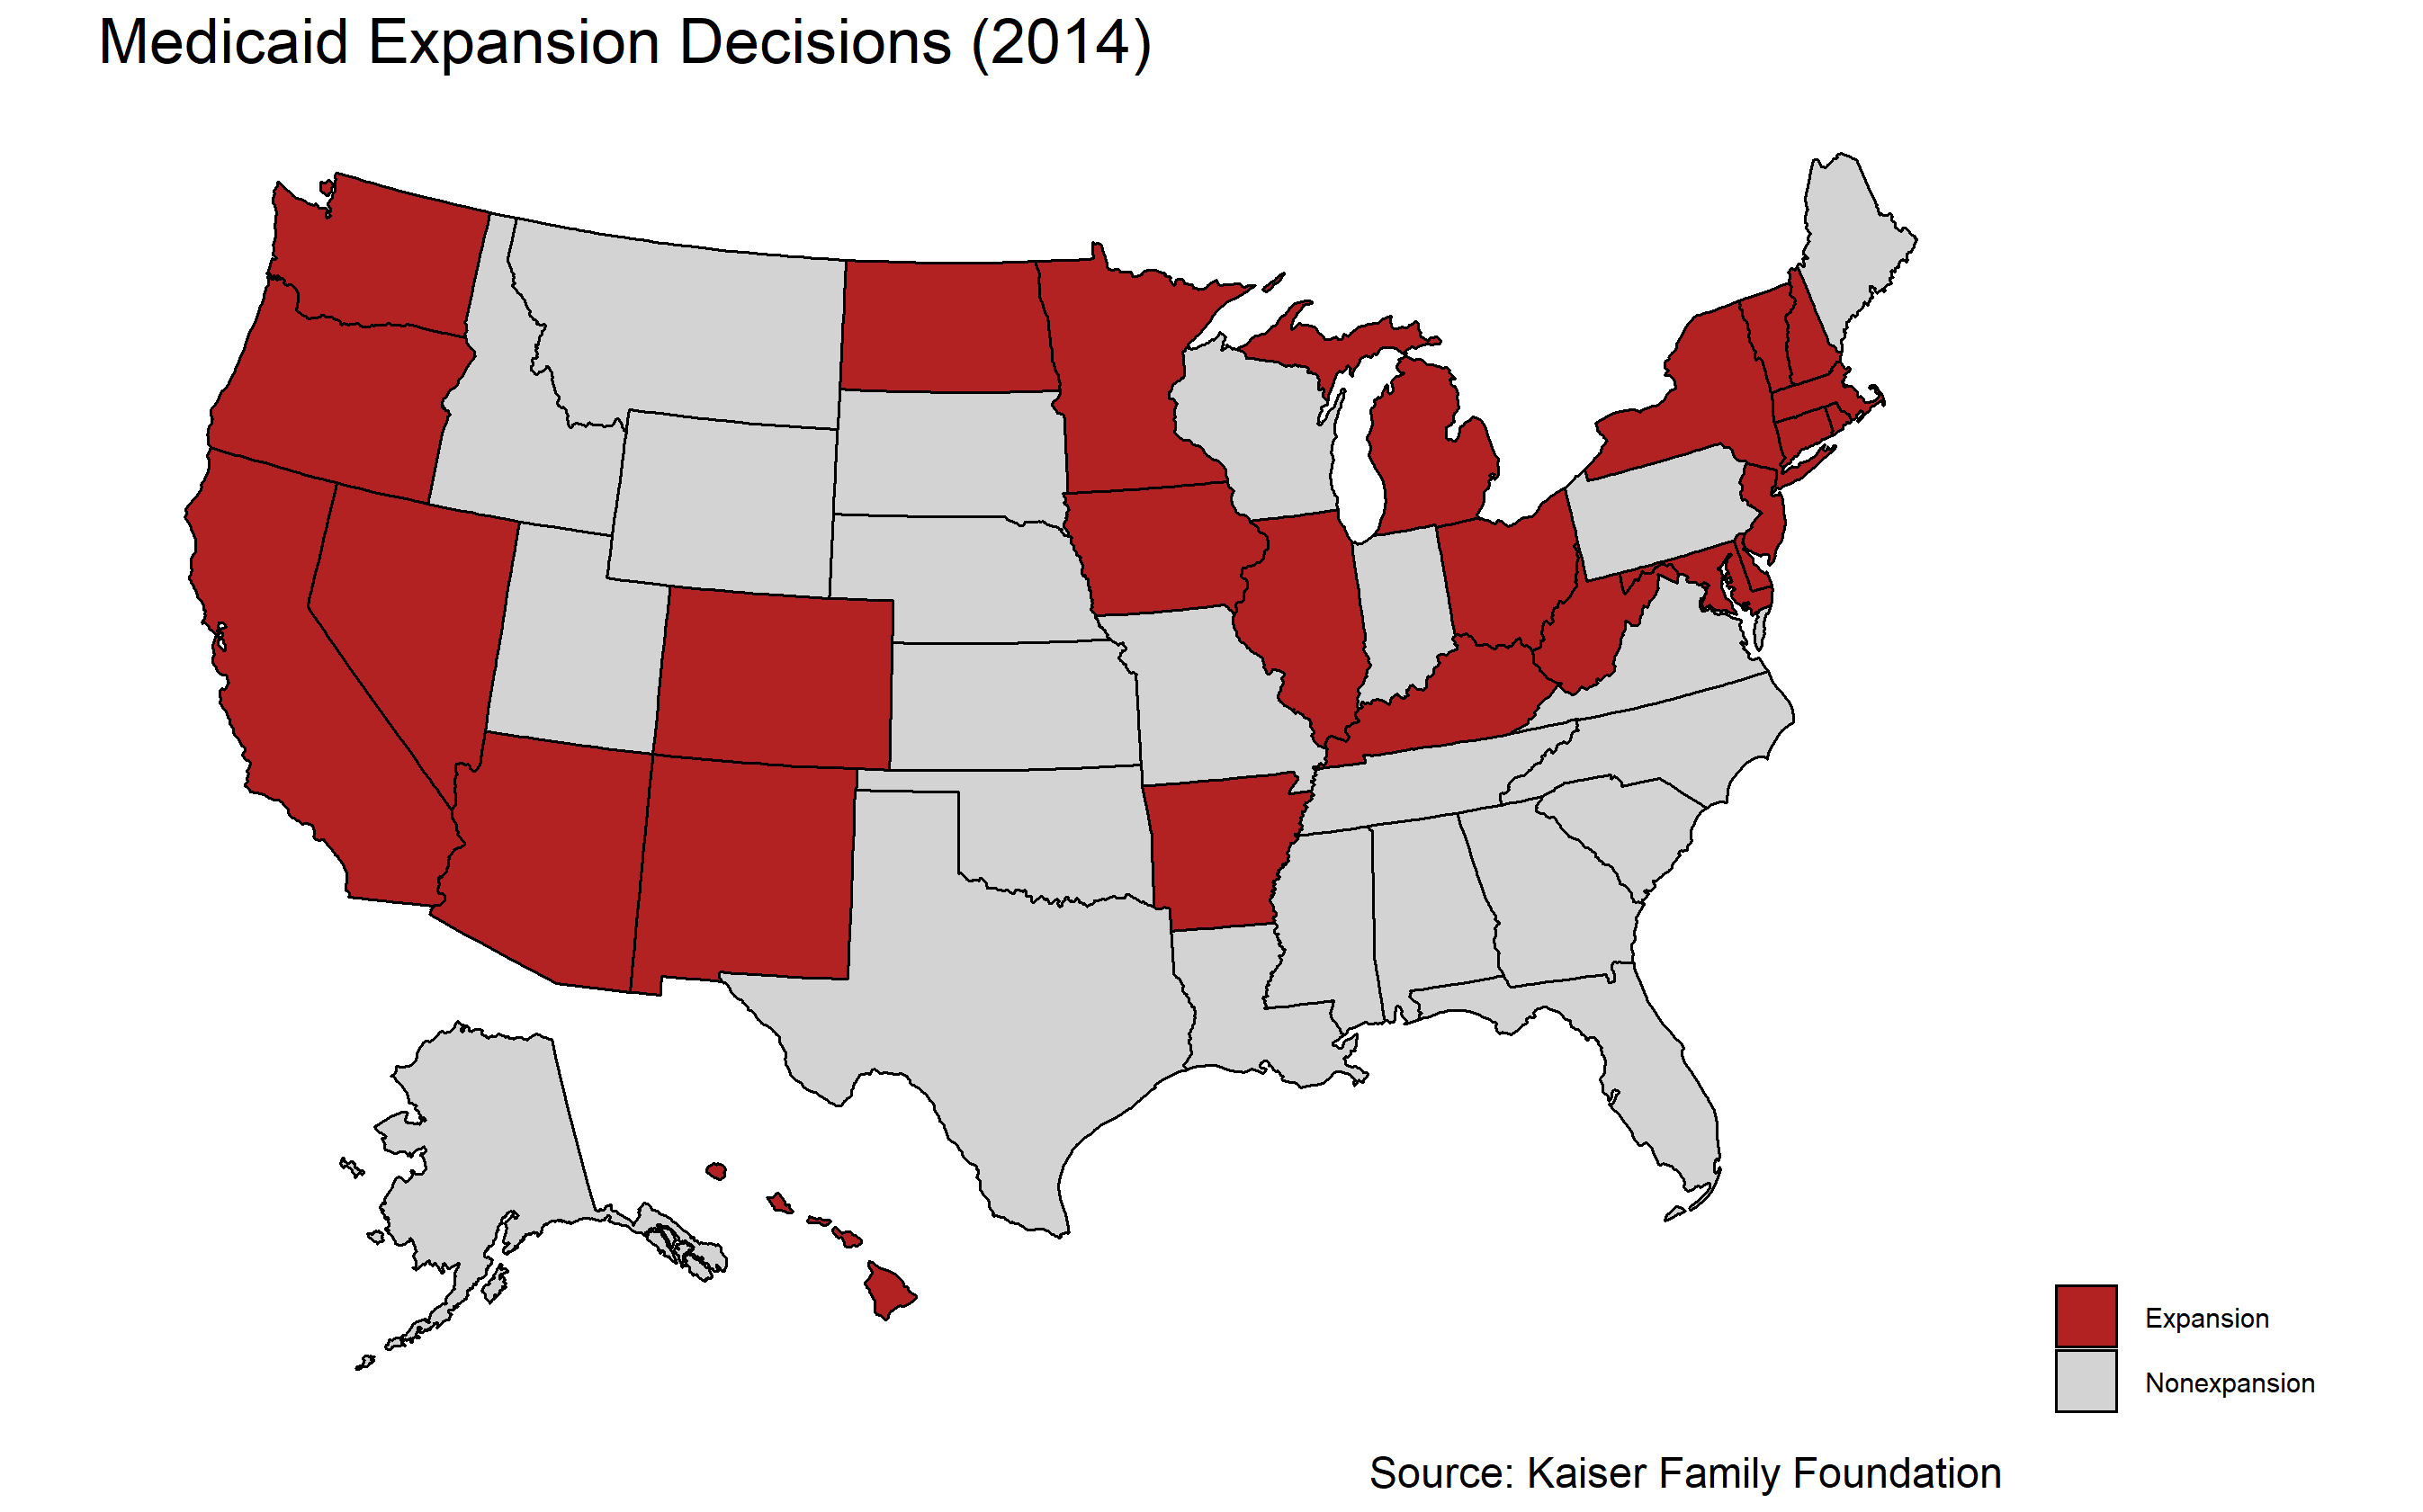
\includegraphics[scale=0.5]{01_Plots/expansion-map.png}
    \end{center}
\end{frame}

\begin{frame}{Background}
    \begin{center}
	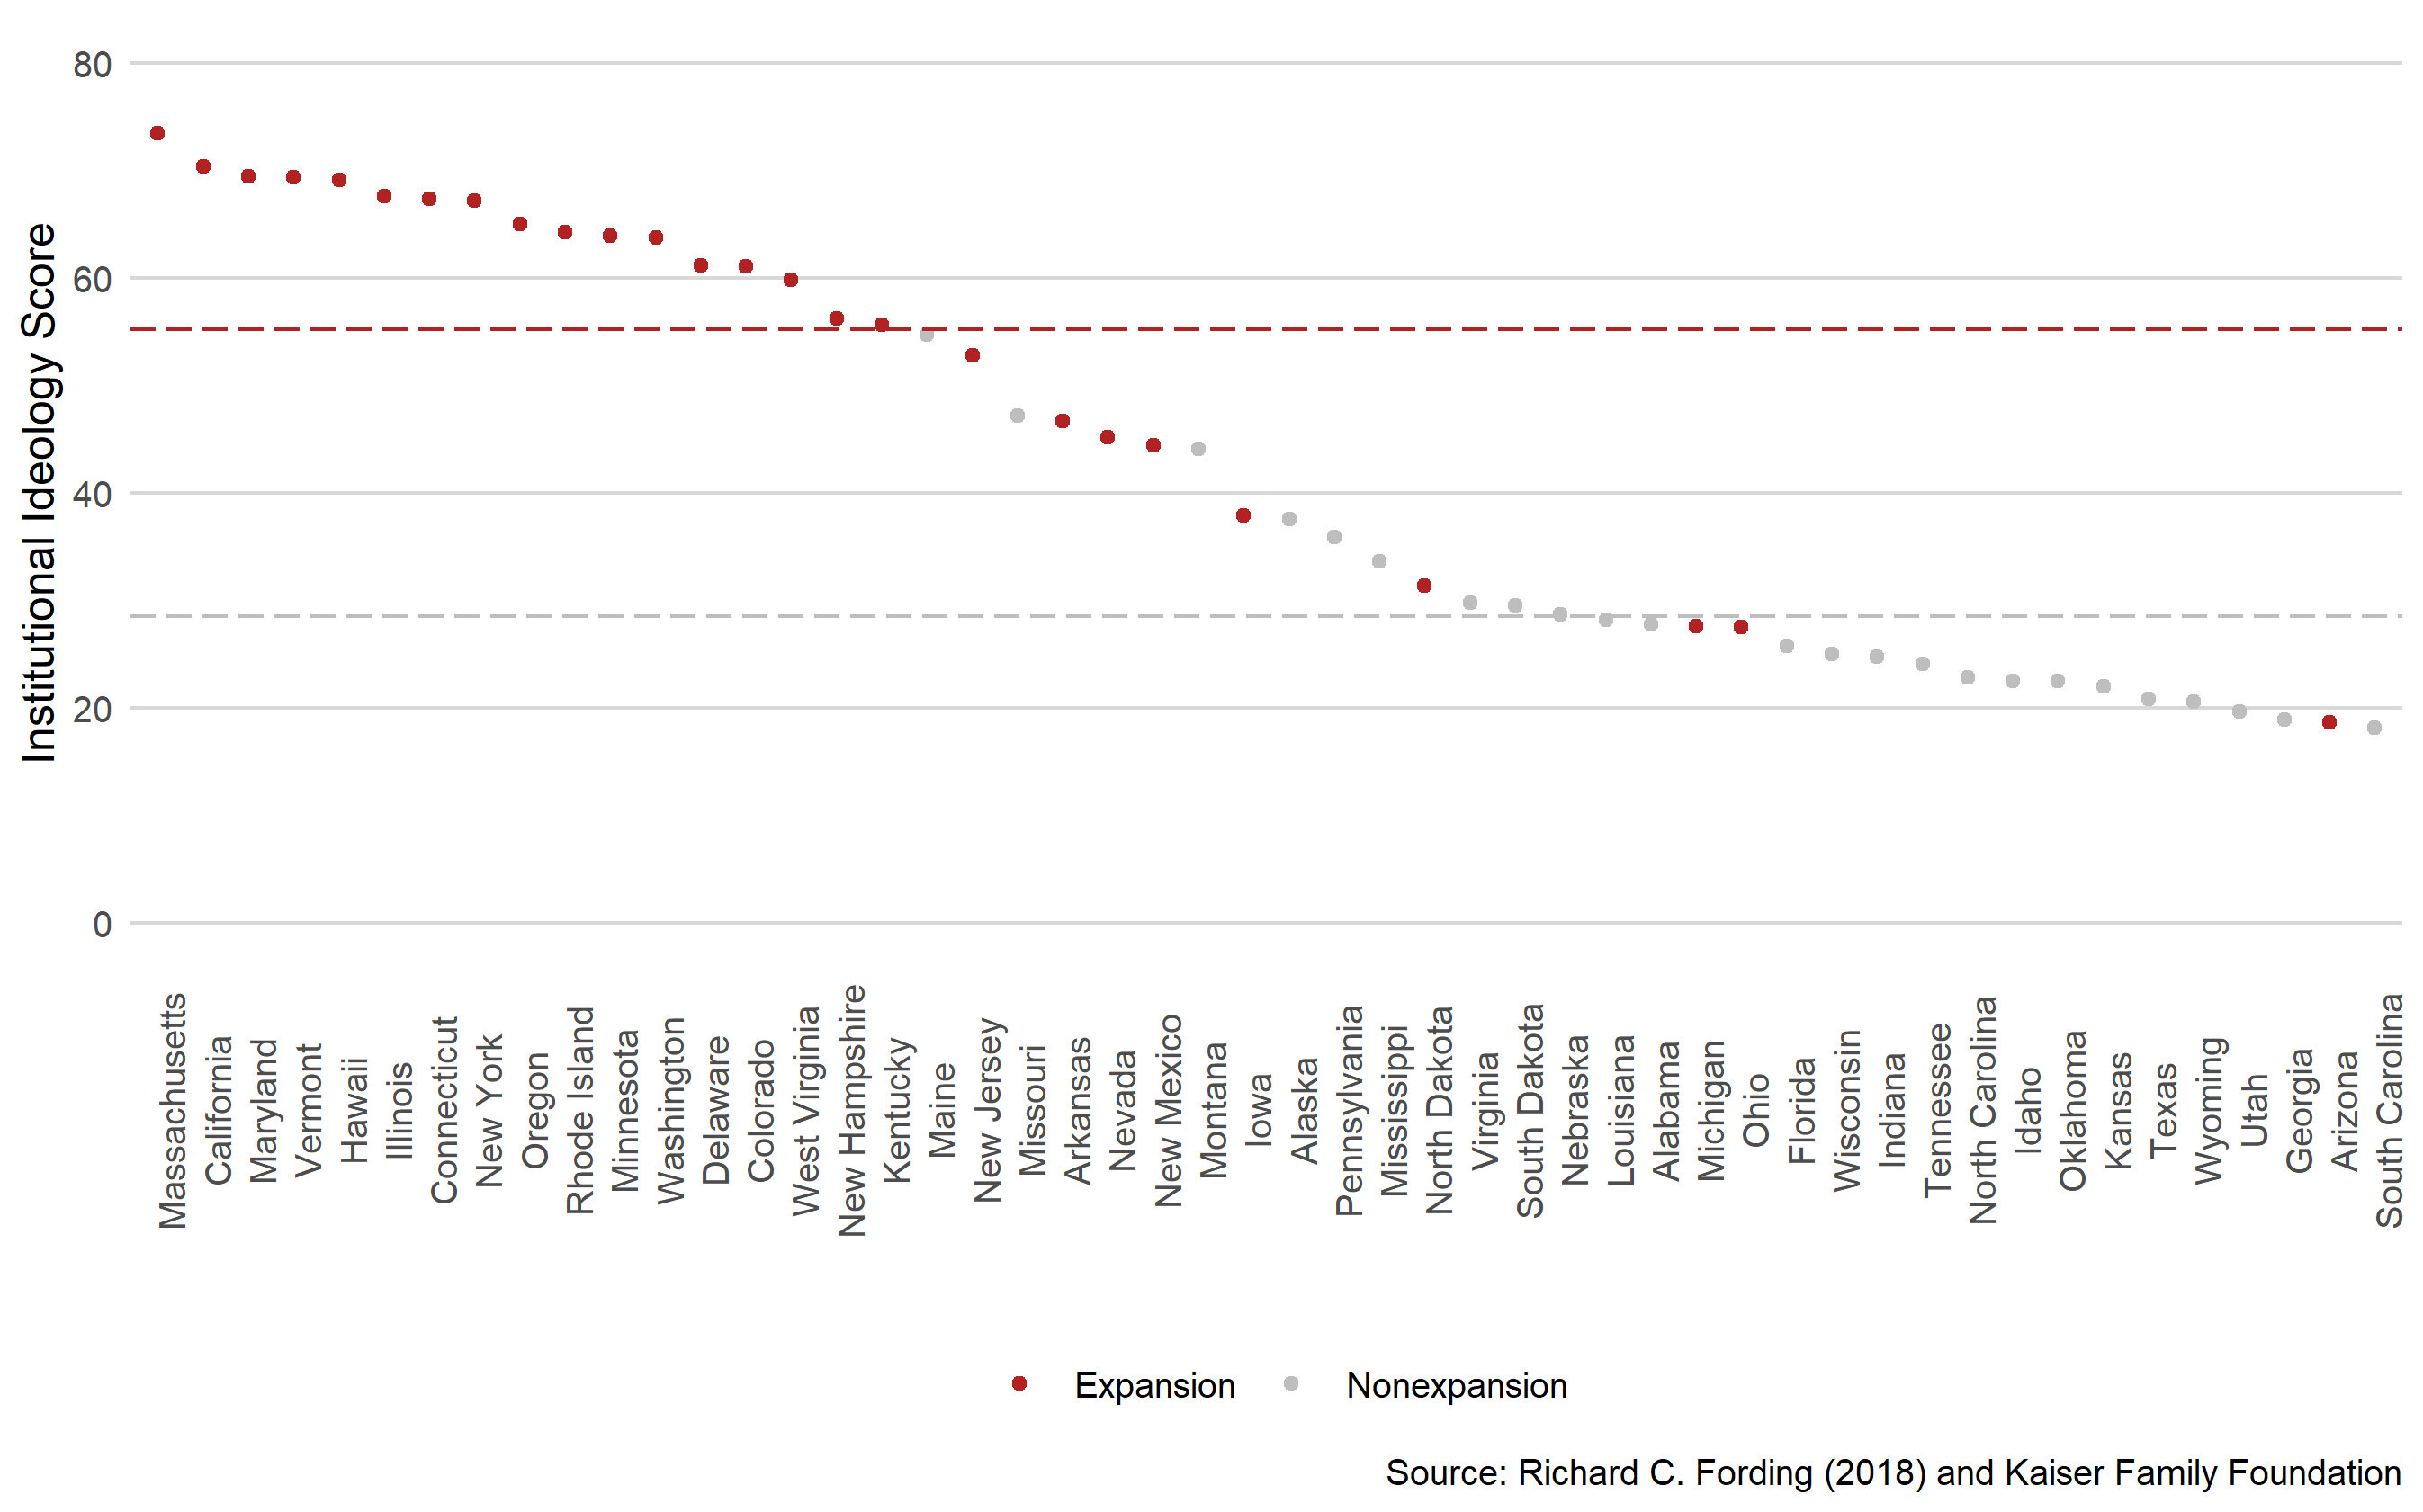
\includegraphics[scale=0.5]{01_Plots/political-expansion-plot.png}
    \end{center}
\end{frame}

\begin{frame}{Motivation}
    \begin{itemize}
    \item Insuring previously uninsured individuals mediates many effects of Medicaid expansion \bigskip
    \item To understand the magnitude of foregone coverage increases due to the 2012 Supreme Court decision \bigskip
    \item To understand the association between governance and Medicaid enrollment in 2014 
    \end{itemize} 
\end{frame}

\begin{frame}{Contributions: Substantive}
\begin{itemize}
    \item We estimate the treatment effect of 2014 Medicaid expansion on non-expansion states \bigskip
    
    \begin{itemize}
        \item We estimate -2.08 percentage point change, 34 percent lower magnitude than ETT from Courtenmanche et al. (2017) \bigskip 
    \end{itemize}

    \item We estimate the association of governance with the change in uninsurance rate \bigskip
    
    \begin{itemize}
        \item We find a negative association between Republican governance and the estimated treatment effect, consistent with Sommers et al. (2012) \bigskip 
    \end{itemize}
    \end{itemize}
\end{frame}

\begin{frame}{Contributions: Methdological}
\begin{itemize}
    \item We outline the assumptions necessary to estimate a ``synthetic treatment'' using longitudinal data \bigskip
    
    \item We generate weights that account for hierarchical data structure \bigskip
    
    \item We account for measurement error in our covariates \bigskip
    \end{itemize}
\end{frame}

\section{Data \& Methods}

\subsection{Target estimand}

\begin{frame}{Target estimand}

$$
N_0^{-1}\sum_{s: A_s = 0} \sum_{c = 1}^{n_s} Y_{sc}^1 - Y_{sc}^0
$$

\begin{itemize}
    \item $Y$ is the uninsurance rate (at the ``county'' level) \bigskip
    \item $A$ is the decision to expand Medicaid (at the state level)   
\end{itemize}
\end{frame}

\subsection{Treatment assignment}

\begin{frame}{Treatment assignment}
    \begin{center}
	\includegraphics[scale=0.6]{medicaid-heterogeneity.png}
    \end{center}
\end{frame}

\begin{frame}{Treatment assignment}
    \begin{center}
	\includegraphics[scale=0.6]{ctrl-grps.png}  
    \end{center}
\end{frame}

\subsection{Identification}

\begin{frame}{Identifying Assumptions}

\begin{itemize}
    \item Consistency \bigskip
    \begin{itemize}
        \item $Y_{sc}^a = Y_{sc} \mid A_s = a$ \bigskip
    \end{itemize}
    \item No anticipatory effects \bigskip
    \begin{itemize}
        \item For $t < T$, $Y_{sct}^0 = Y_{sct}$ \bigskip
    \end{itemize}
    \item Positivity \bigskip
    \item No unmeasured confounding \bigskip
    \begin{itemize}
        \item $Y^a_{sc} \perp A_s | X_{sc}$ \bigskip 
    \end{itemize}
\end{itemize}

\end{frame}

\begin{frame}{Covariates}
\begin{itemize}
    \item Uninsurance rates (2011-13) \bigskip
    \item Unemployment rates (2011-13) \bigskip
    \item ``Time-invariant'' demographics (2011-13 averages) \bigskip
    \begin{itemize}
        \item Age, sex, race, ethnicity, disability, foreign born, citizenship, education, income-to-poverty ratio, urban residence, married, children \bigskip
    \end{itemize}
    \item Political partisan composition \bigskip
    \begin{itemize}
        \item Republican governor, Republican lower chamber control, Republican total control
    \end{itemize}
\end{itemize}
\end{frame}

\begin{frame}{Data Source}
    \begin{itemize}
    \item American Community Survey (ACS) microdata from 2011-2014 \bigskip 
    \item Approximately three million individuals surveyed annually from across the United States \bigskip 
    \item Each individual has an associated survey weight and 80 sets of replicate survey weights \bigskip 
    \item Aggregate data to consistent public use microdata area (CPUMA) level
    \end{itemize}
\end{frame}   

\begin{frame}{Problem: measurement error in covariates}
    \begin{itemize}
        \item All of our covariates are estimates \bigskip
        \begin{itemize}
            \item We observe $W_{sc}$ \bigskip
            \item We need $X_{sc}$ \bigskip
        \end{itemize}
        \item This is a measurement error problem
    \end{itemize}
\end{frame}

\begin{frame}{Parametric assumptions}
    \begin{itemize}
        \item Linearity of outcome model \bigskip
        \item Linearity of $X_{cs}$ in $W_{cs}$ 
    \end{itemize}
\end{frame}

\begin{frame}{Estimation}

\end{frame}

\subsection{Inference}

\begin{frame}{Inference}

\end{frame}

\section{Results}

\subsection{Covariate Balance}

\begin{frame}{Covariate Balance}
    \begin{center}
	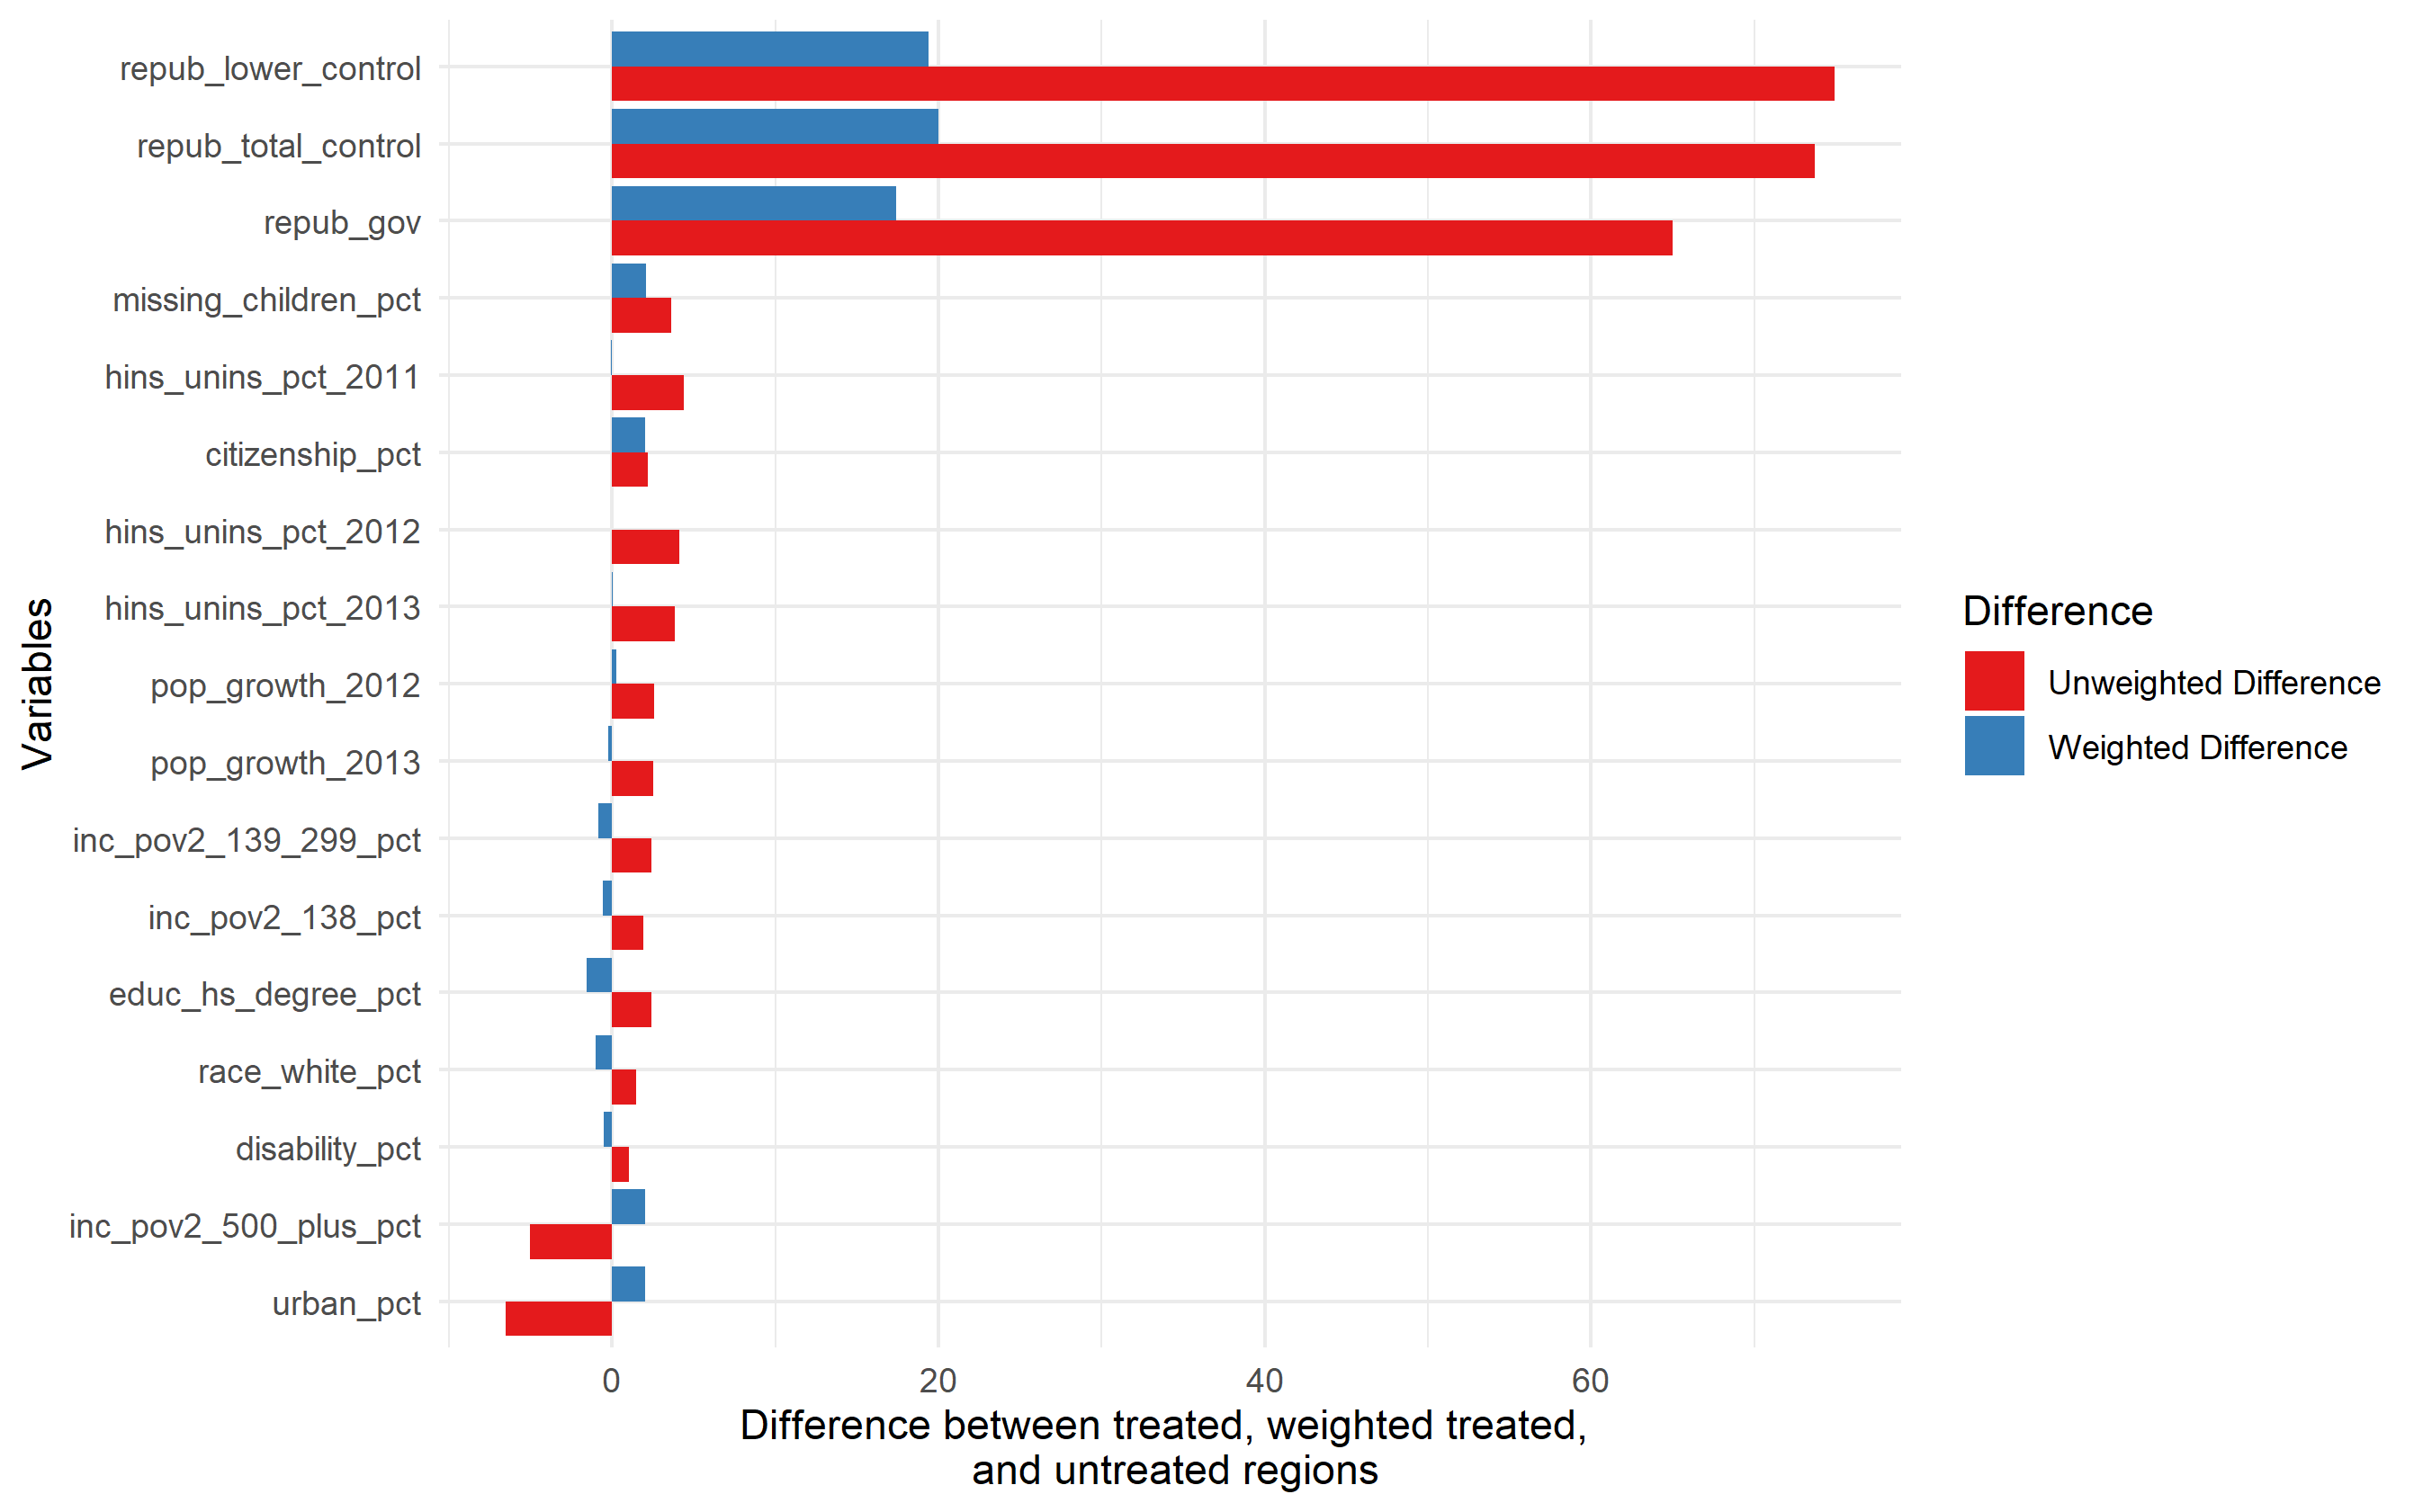
\includegraphics[scale=0.5]{01_Plots/balance-plot-etu.png}
    \end{center}
\end{frame}

\subsection{Primary Results}

\begin{frame}{Results}

\begin{table}[ht]
\begin{tabular}{llrll}
  \toprule
Estimator & Estimate & 95 percent CI (lower, upper)\\ 
  \midrule
  BC-HSBW & -2.14 & (-3.57, -0.71) \\ 
  H-SBW & -2.00 & (-3.59, -0.40) \\ 
  BC-SBW & -1.89 & (-3.06, -0.73) \\ 
  SBW & -1.81 & (-3.60, -0.02) \\ 
   \bottomrule
\end{tabular}
\caption{Primary point estimates and confidence intervals}
\label{tab:confintmain}
\end{table}

\end{frame}

\begin{frame}{Heterogeneity across covariate groups}
\begin{center}
	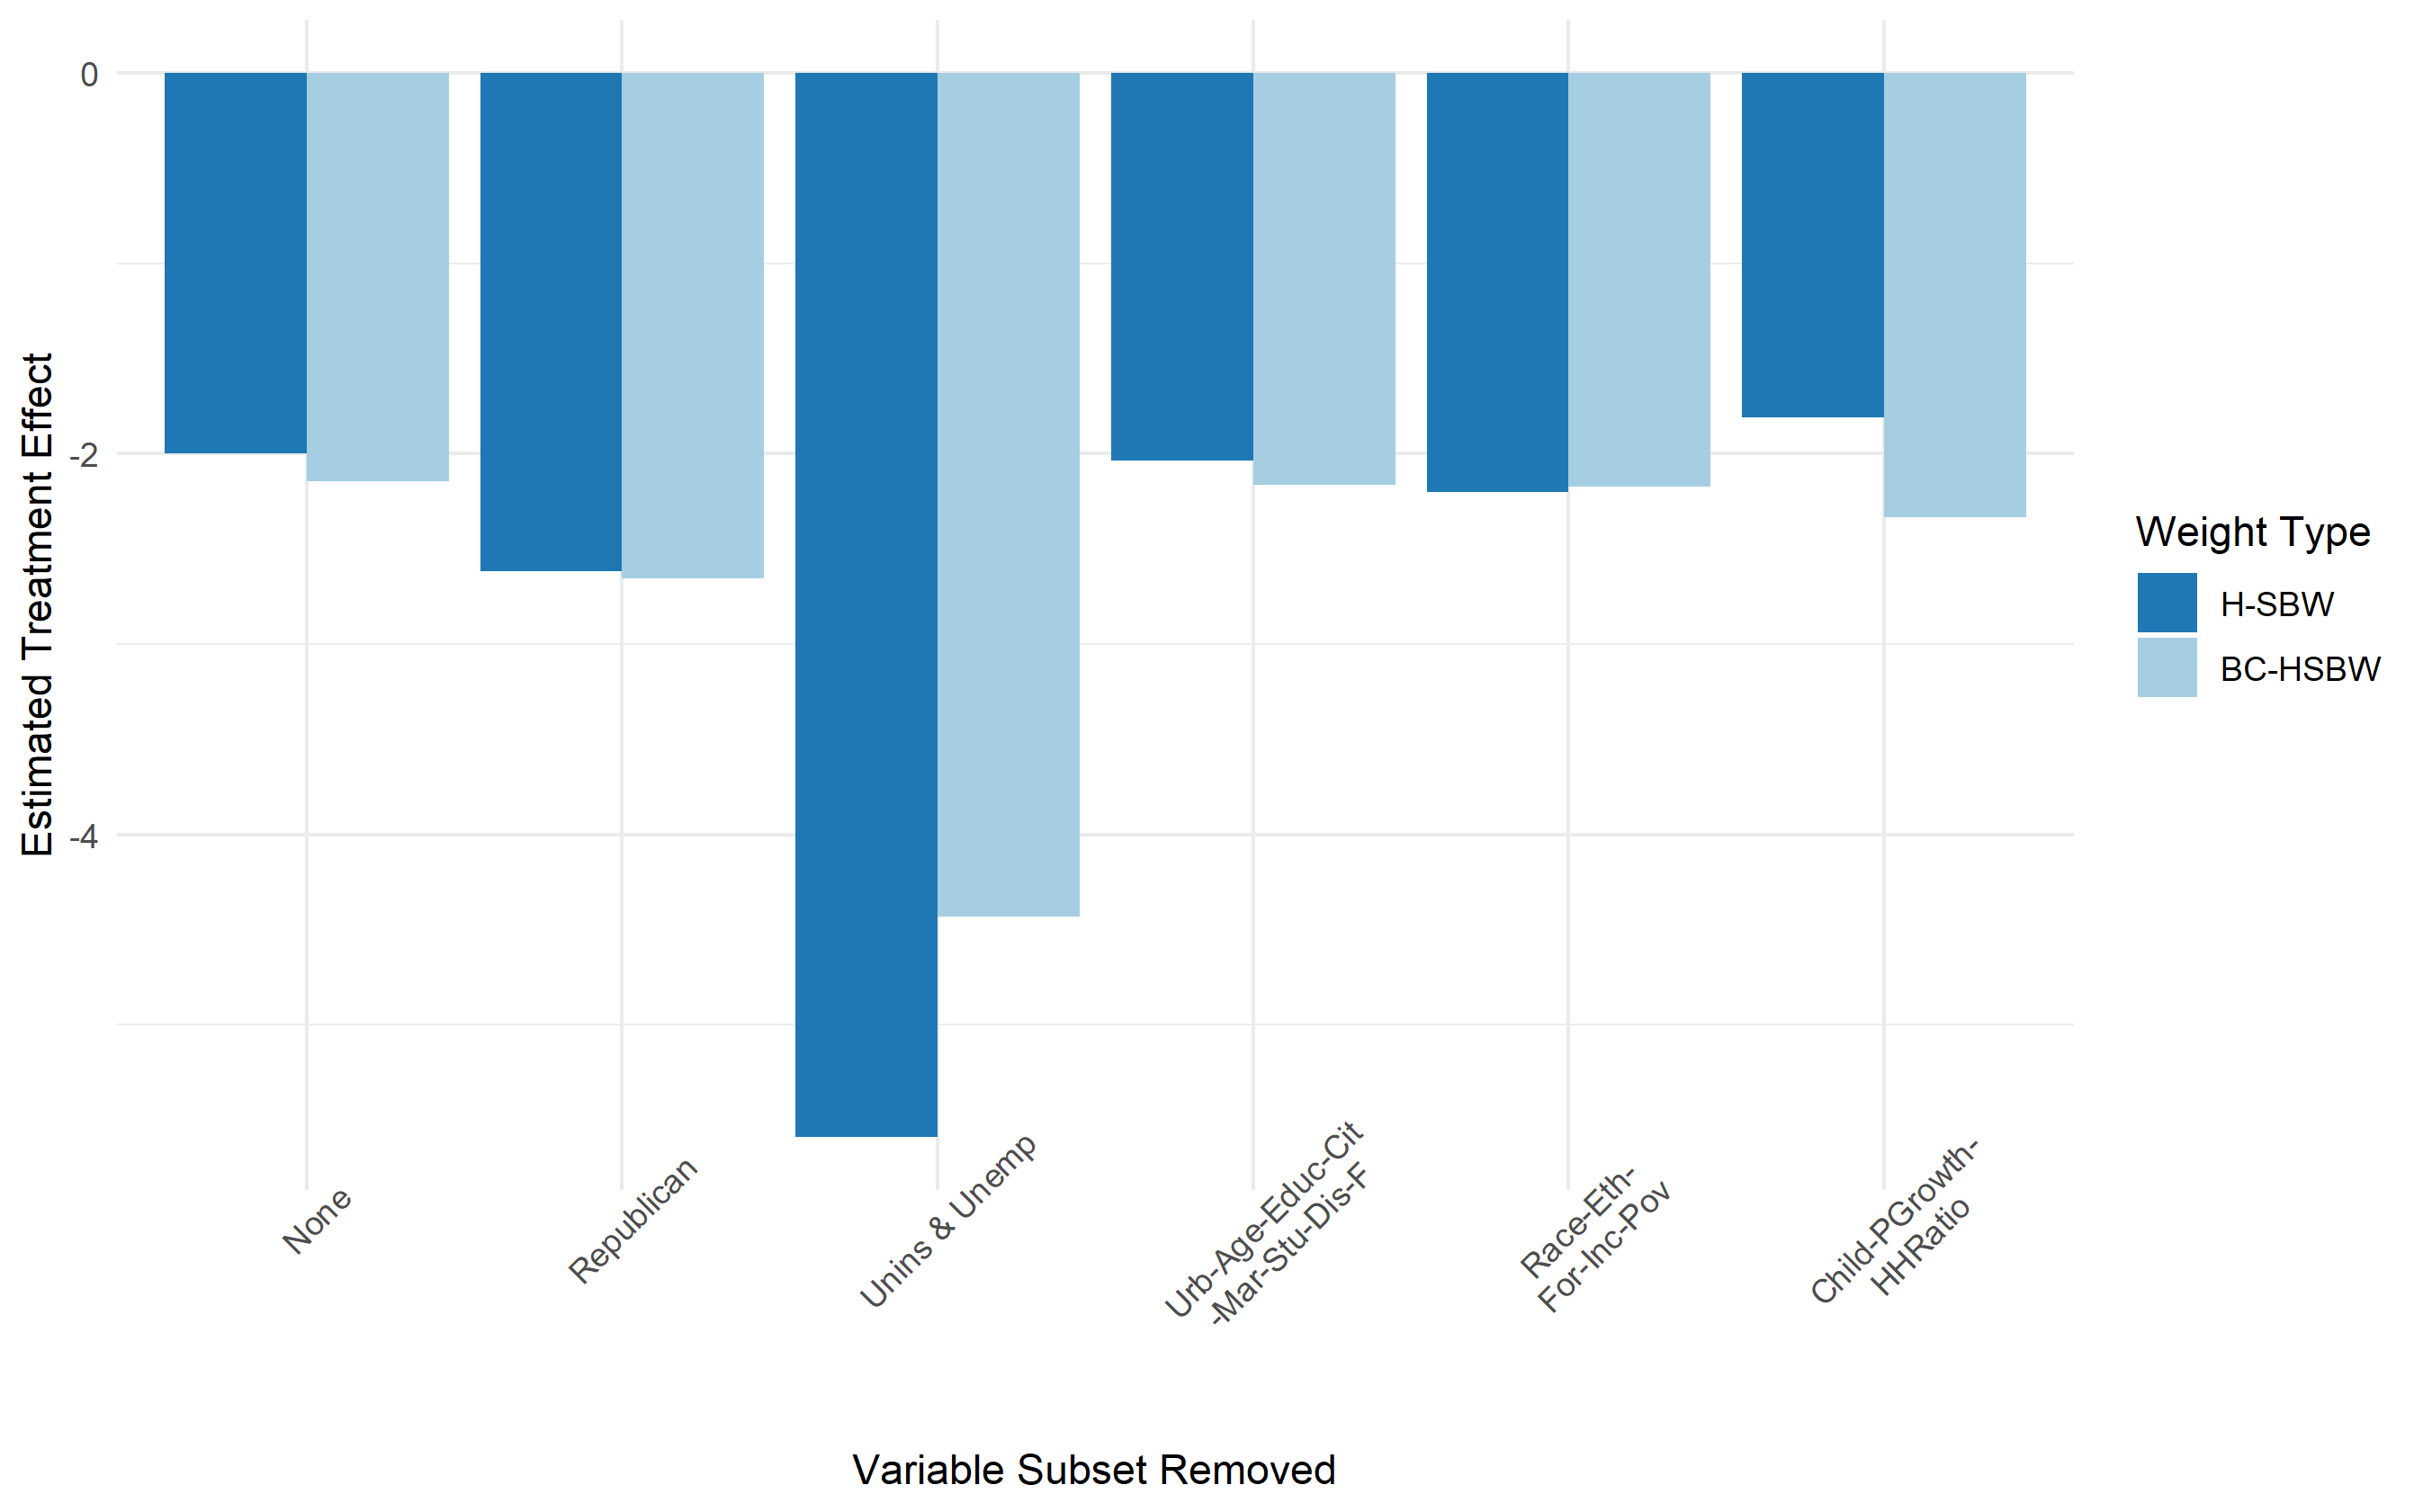
\includegraphics[scale=0.5]{01_Plots/loo-covariates-main-c1.png}
\end{center}
\end{frame}

\begin{frame}{Republican governance removal}
\begin{center}
	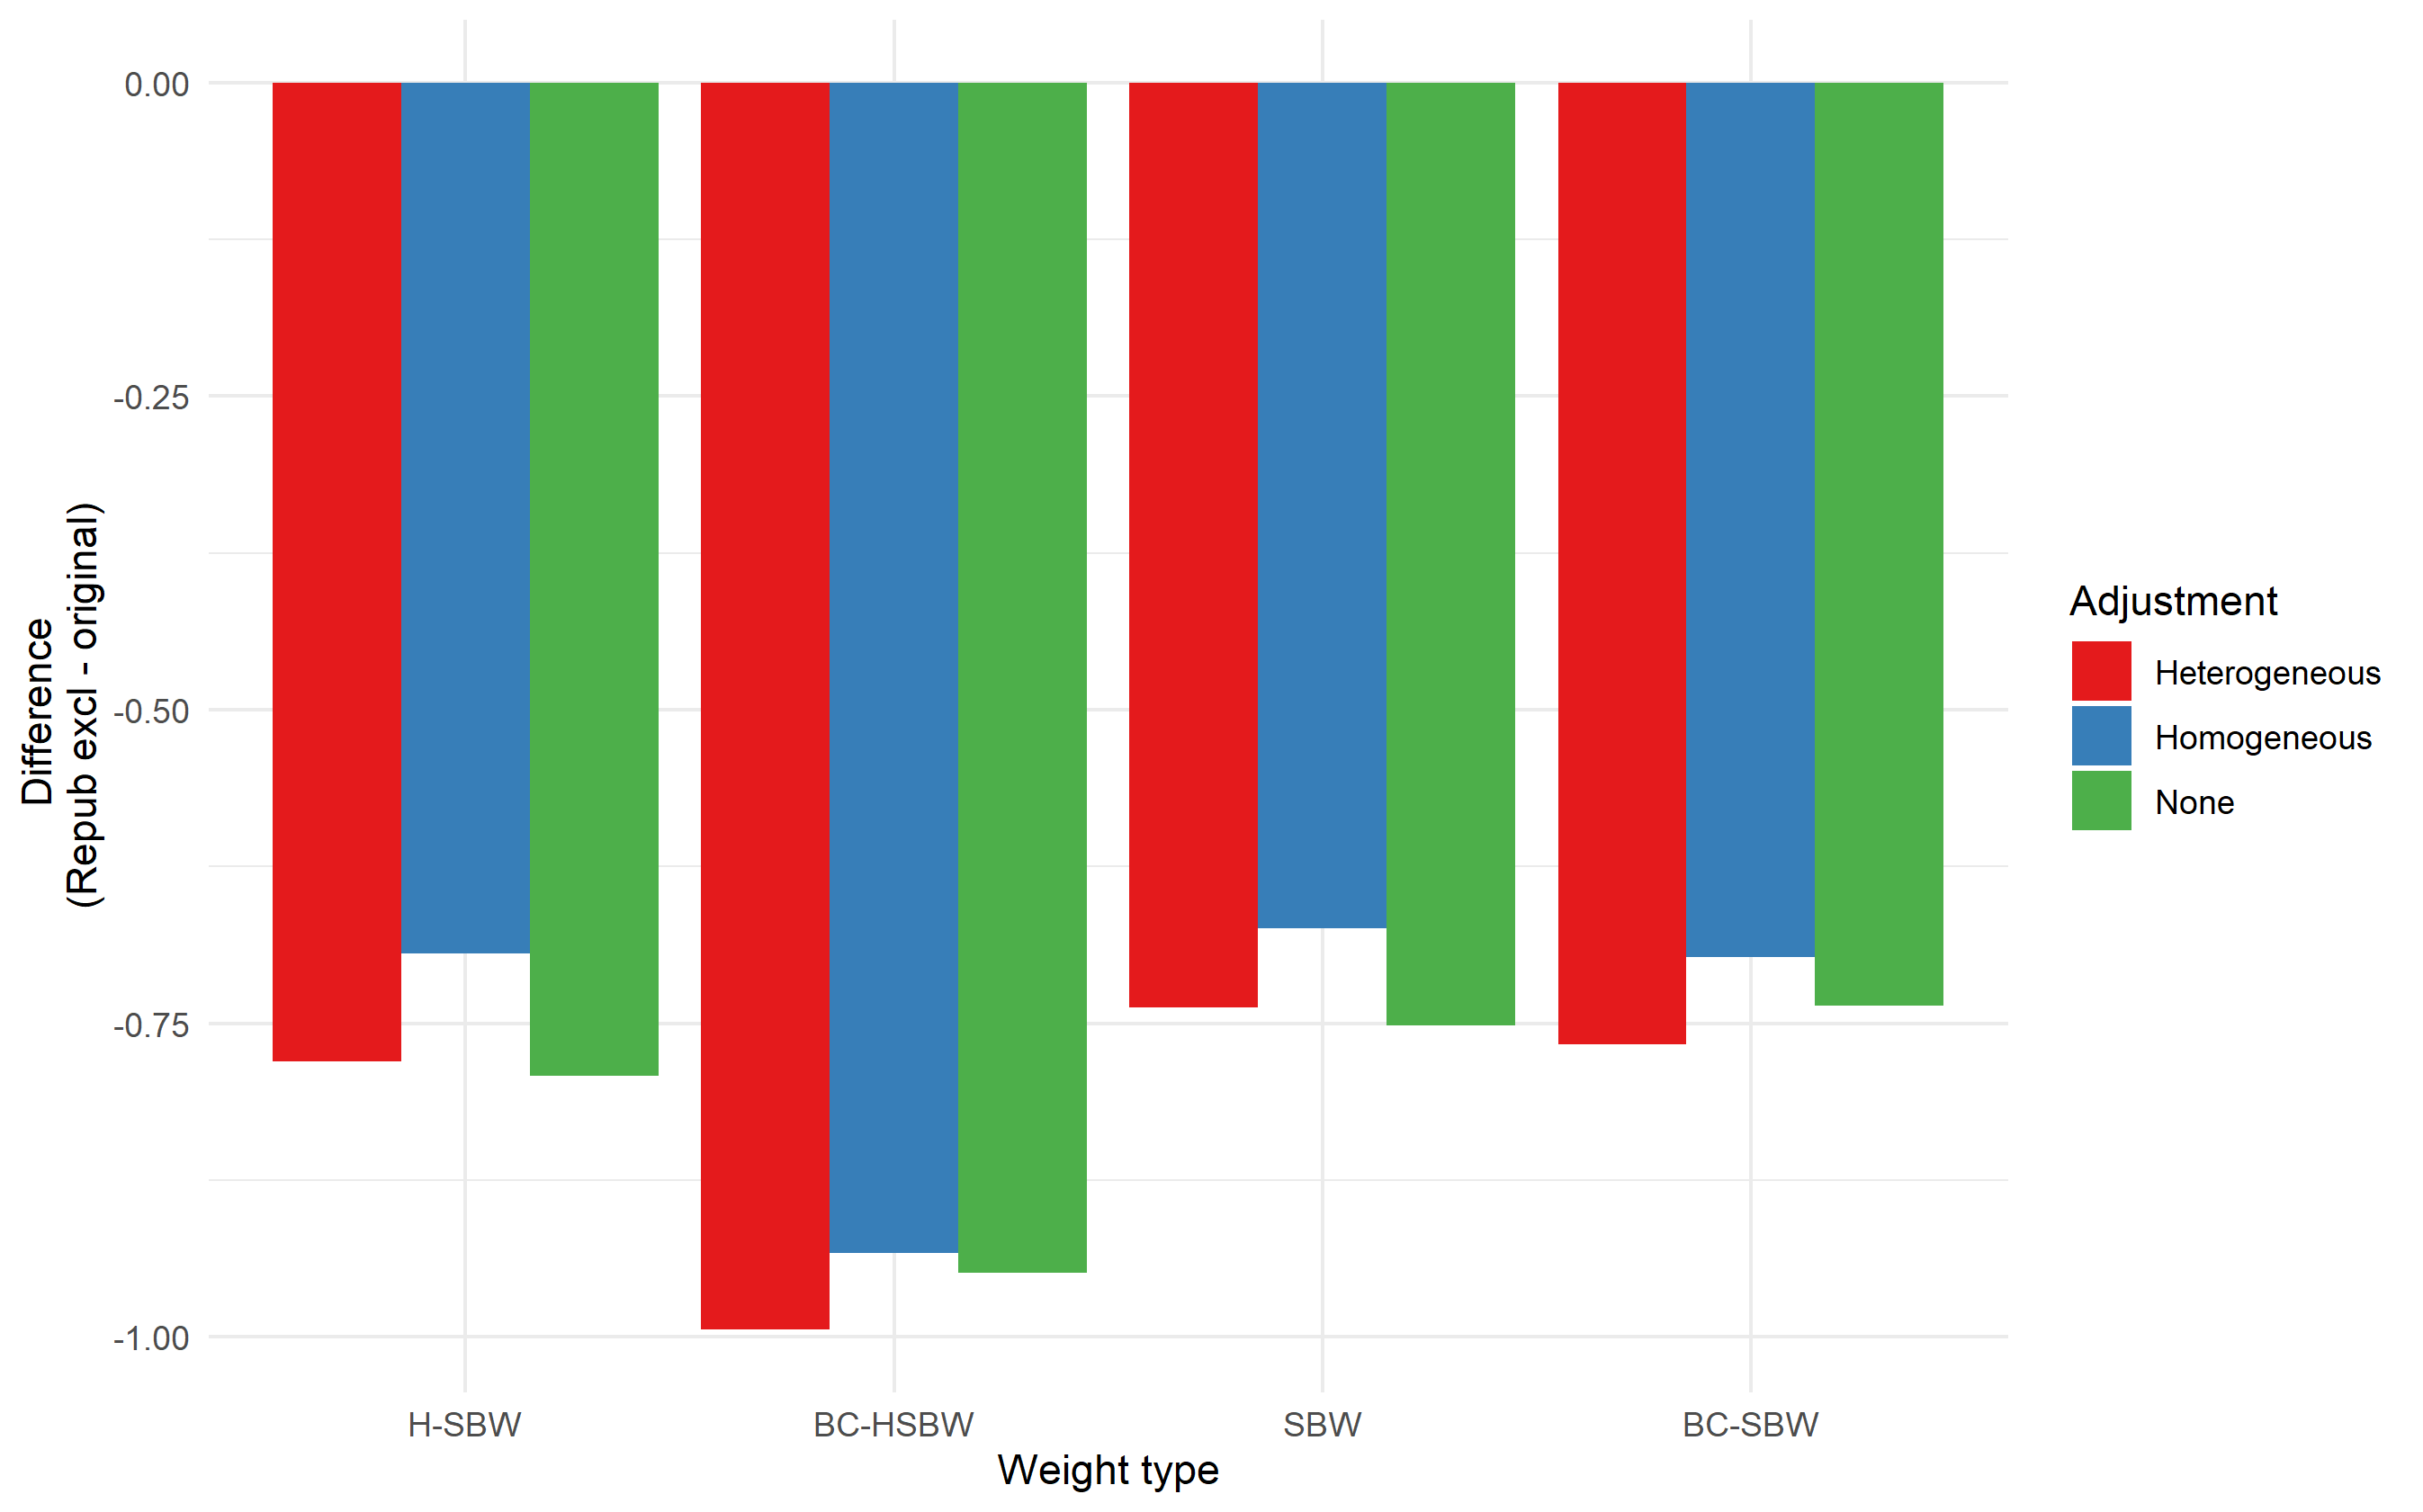
\includegraphics[scale=0.5]{01_Plots/repub-diff-c1-robustness.png}
\end{center}
\end{frame}

\begin{frame}{Leave-one-out-state estimates}
    \begin{center}
	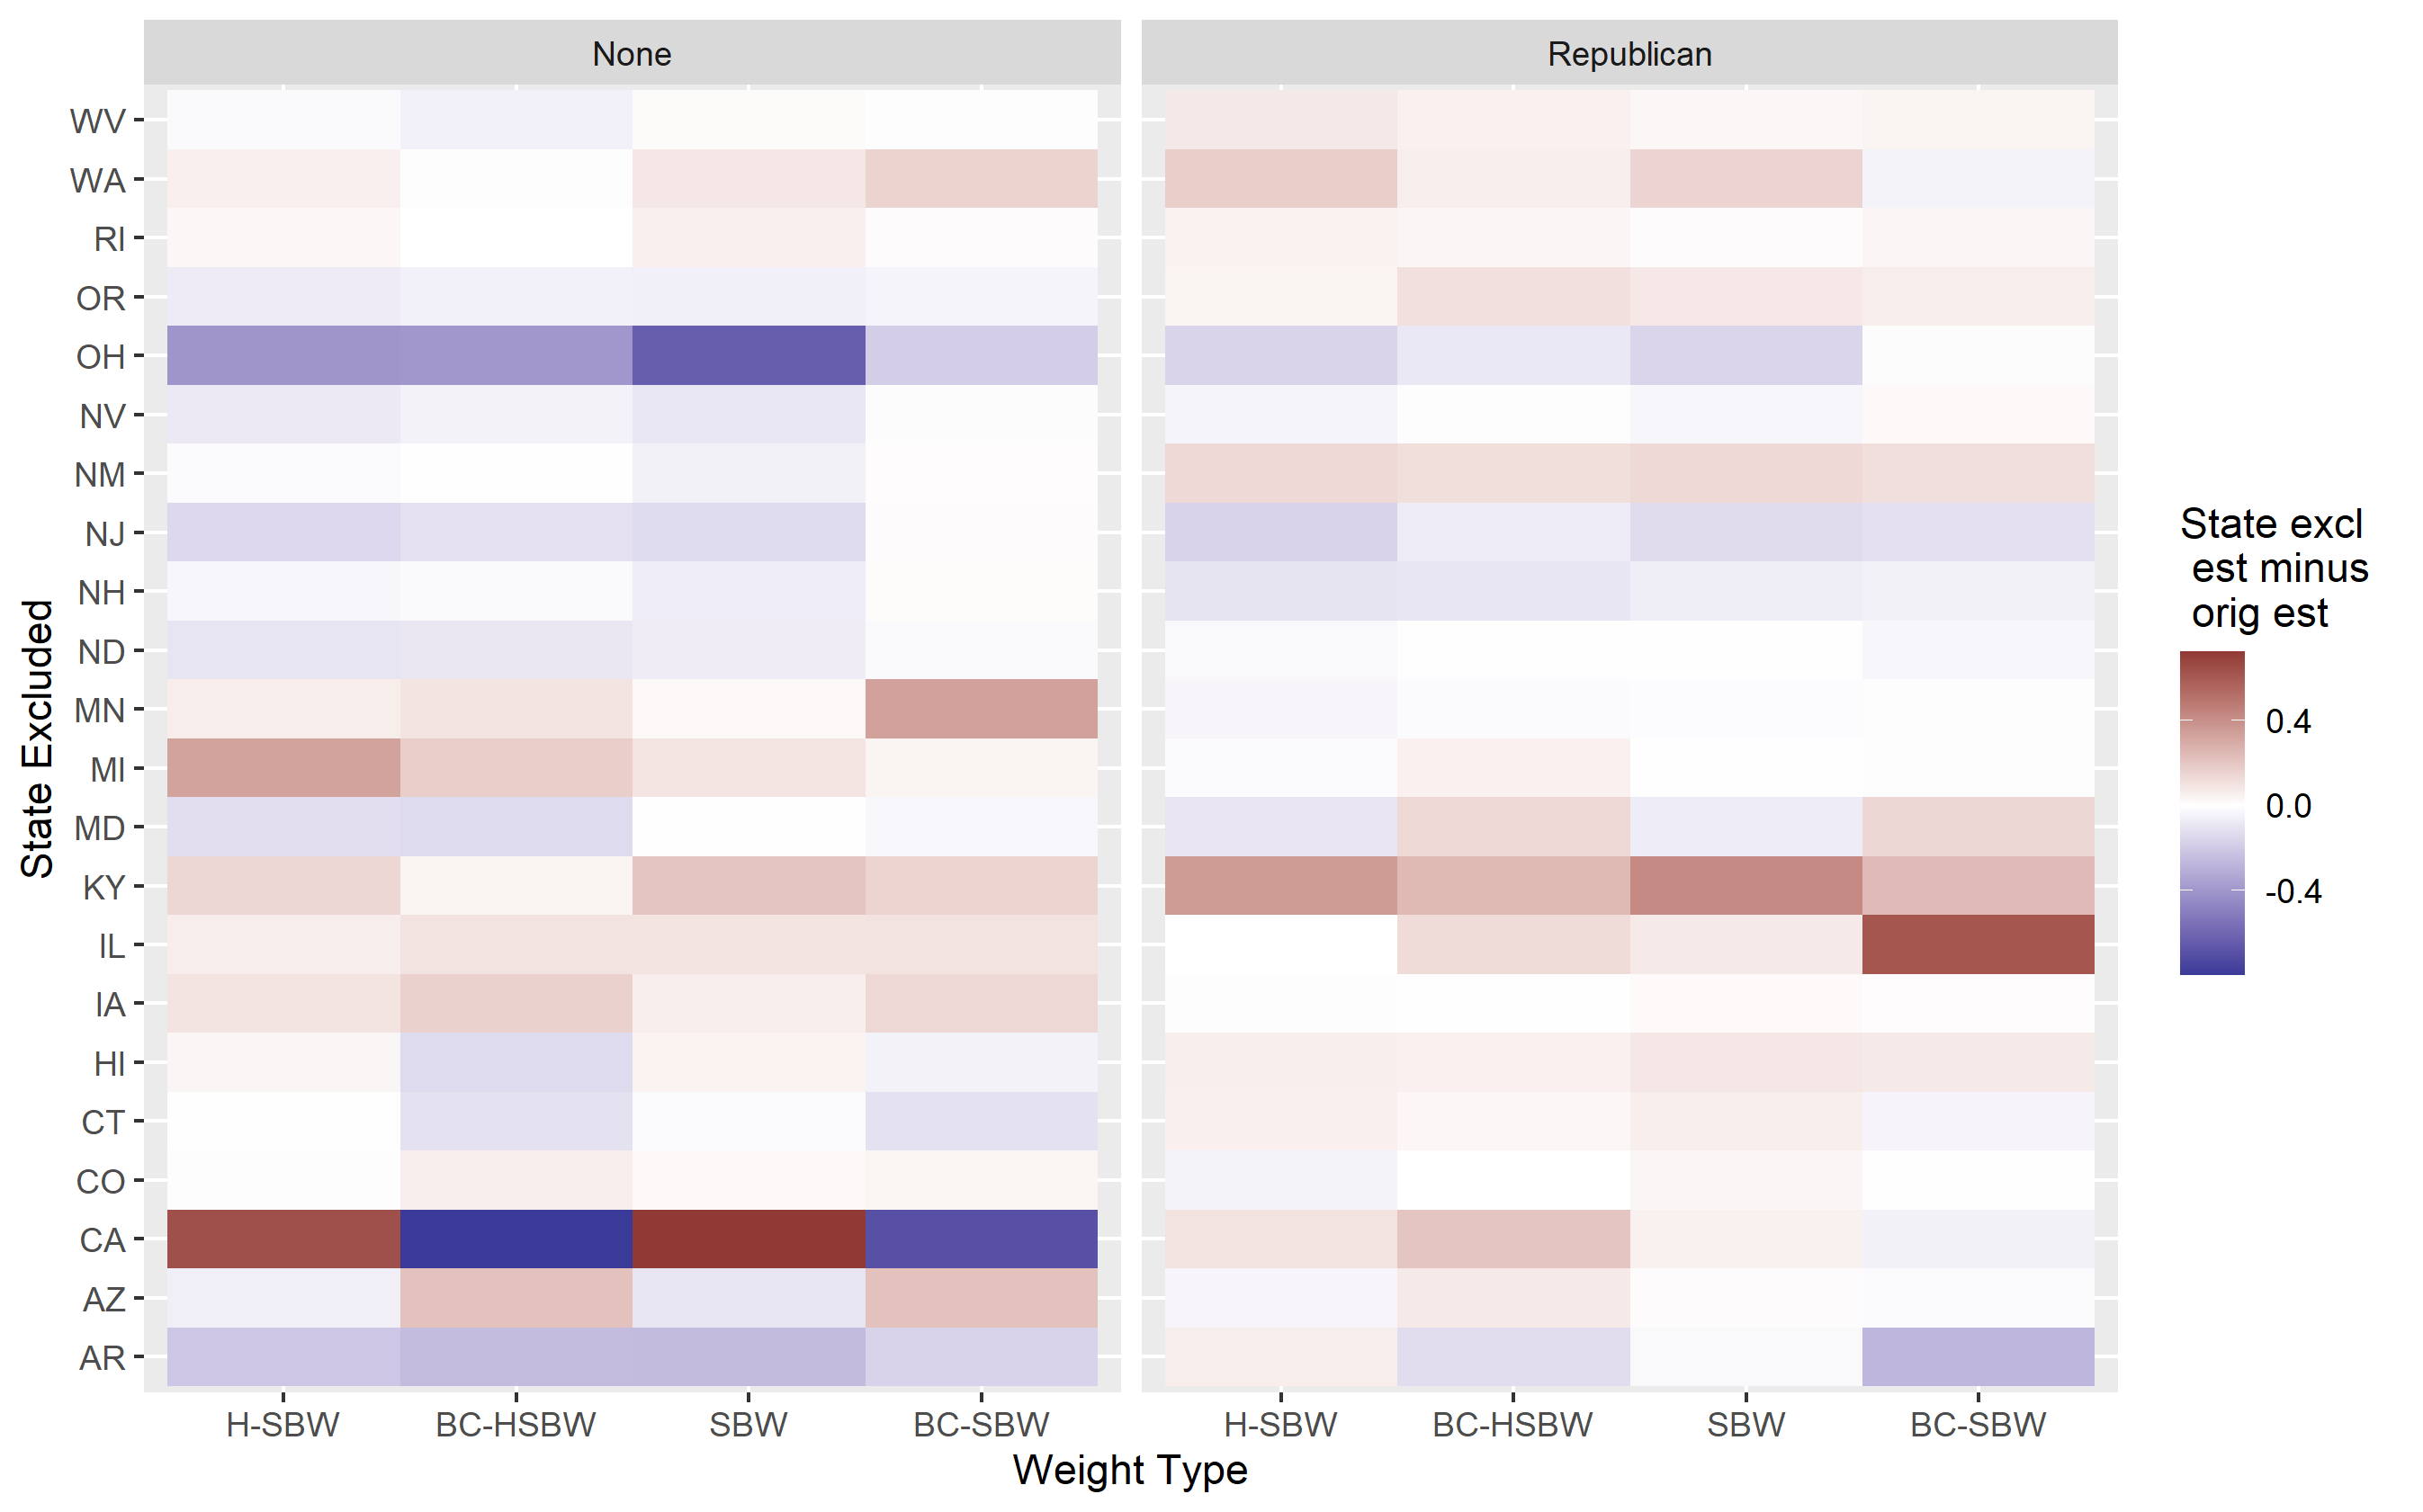
\includegraphics[scale=0.5]{01_Plots/c1-loostate-sensitivity.png}
    \end{center}
\end{frame}

\subsection{Sensitivity analyses: no anticipatory treatment effects}

\begin{frame}{Sensitivity analysis: no anticipatory treatment effects}
    \begin{center}
	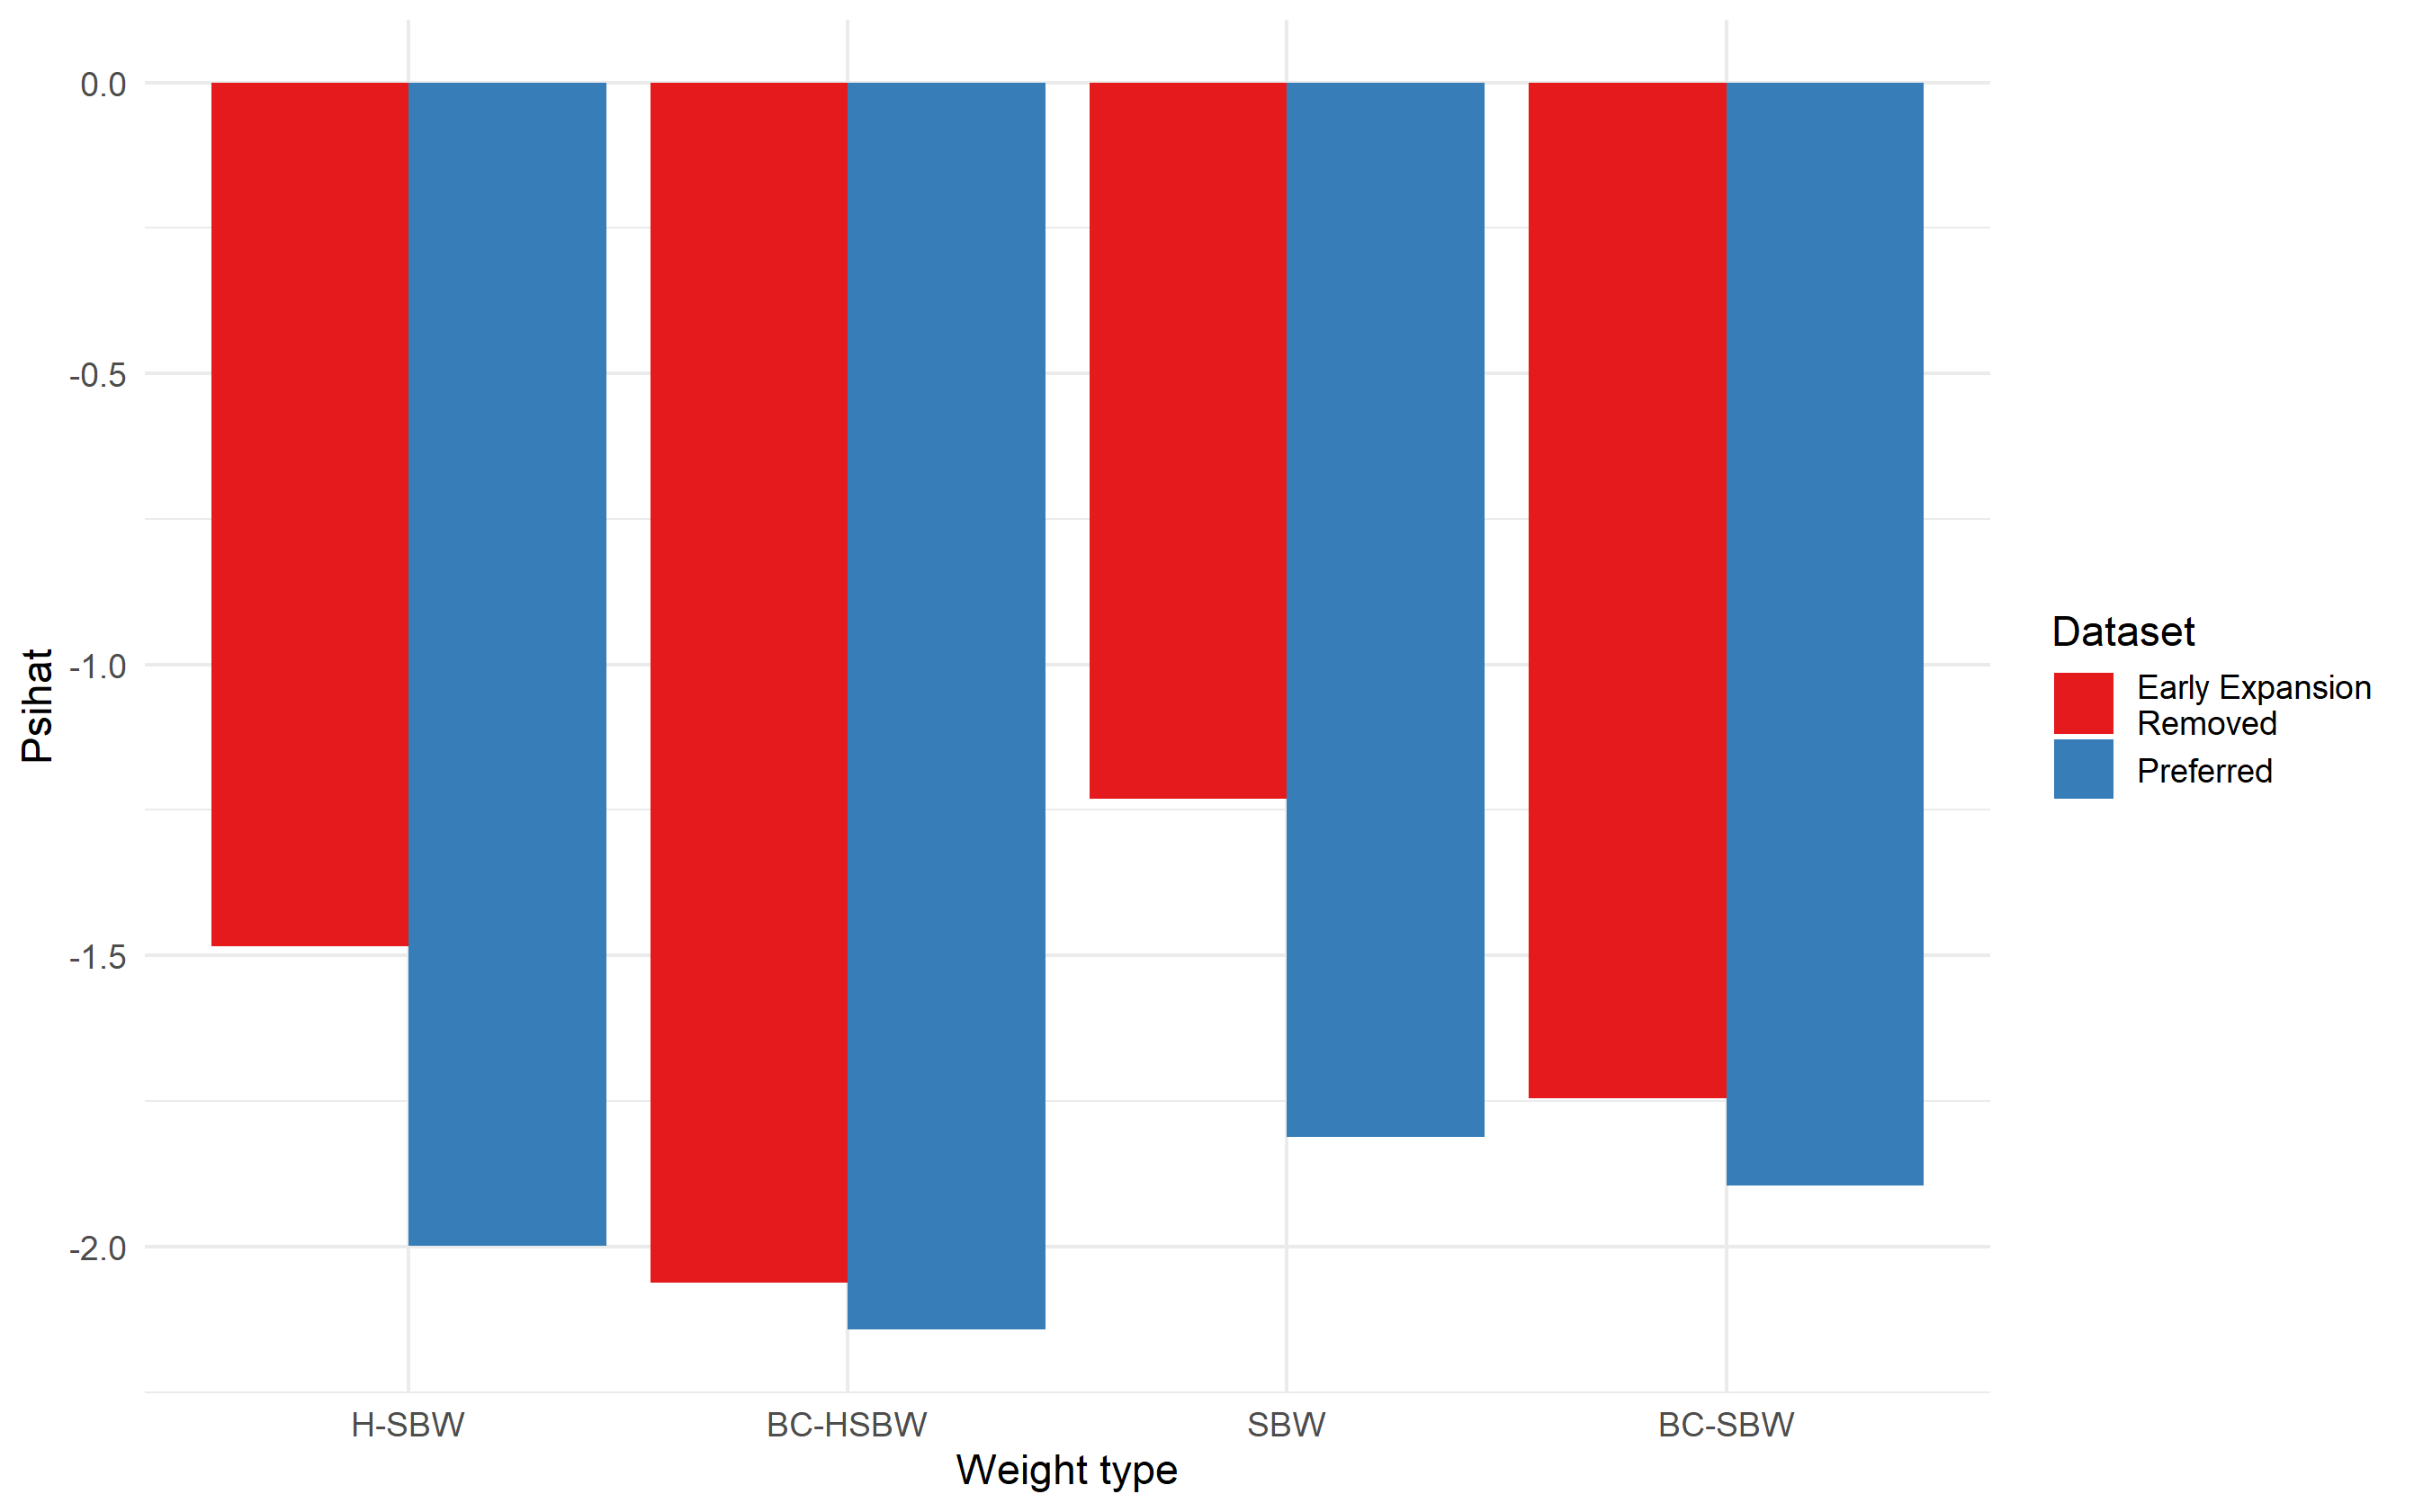
\includegraphics[scale=0.5]{01_Plots/point-estimates-sigmai-c1c2-comparison.png}
    \end{center}
\end{frame}

\begin{frame}{Sensitivity analysis: no anticipatory treatment effects}
    \begin{center}
	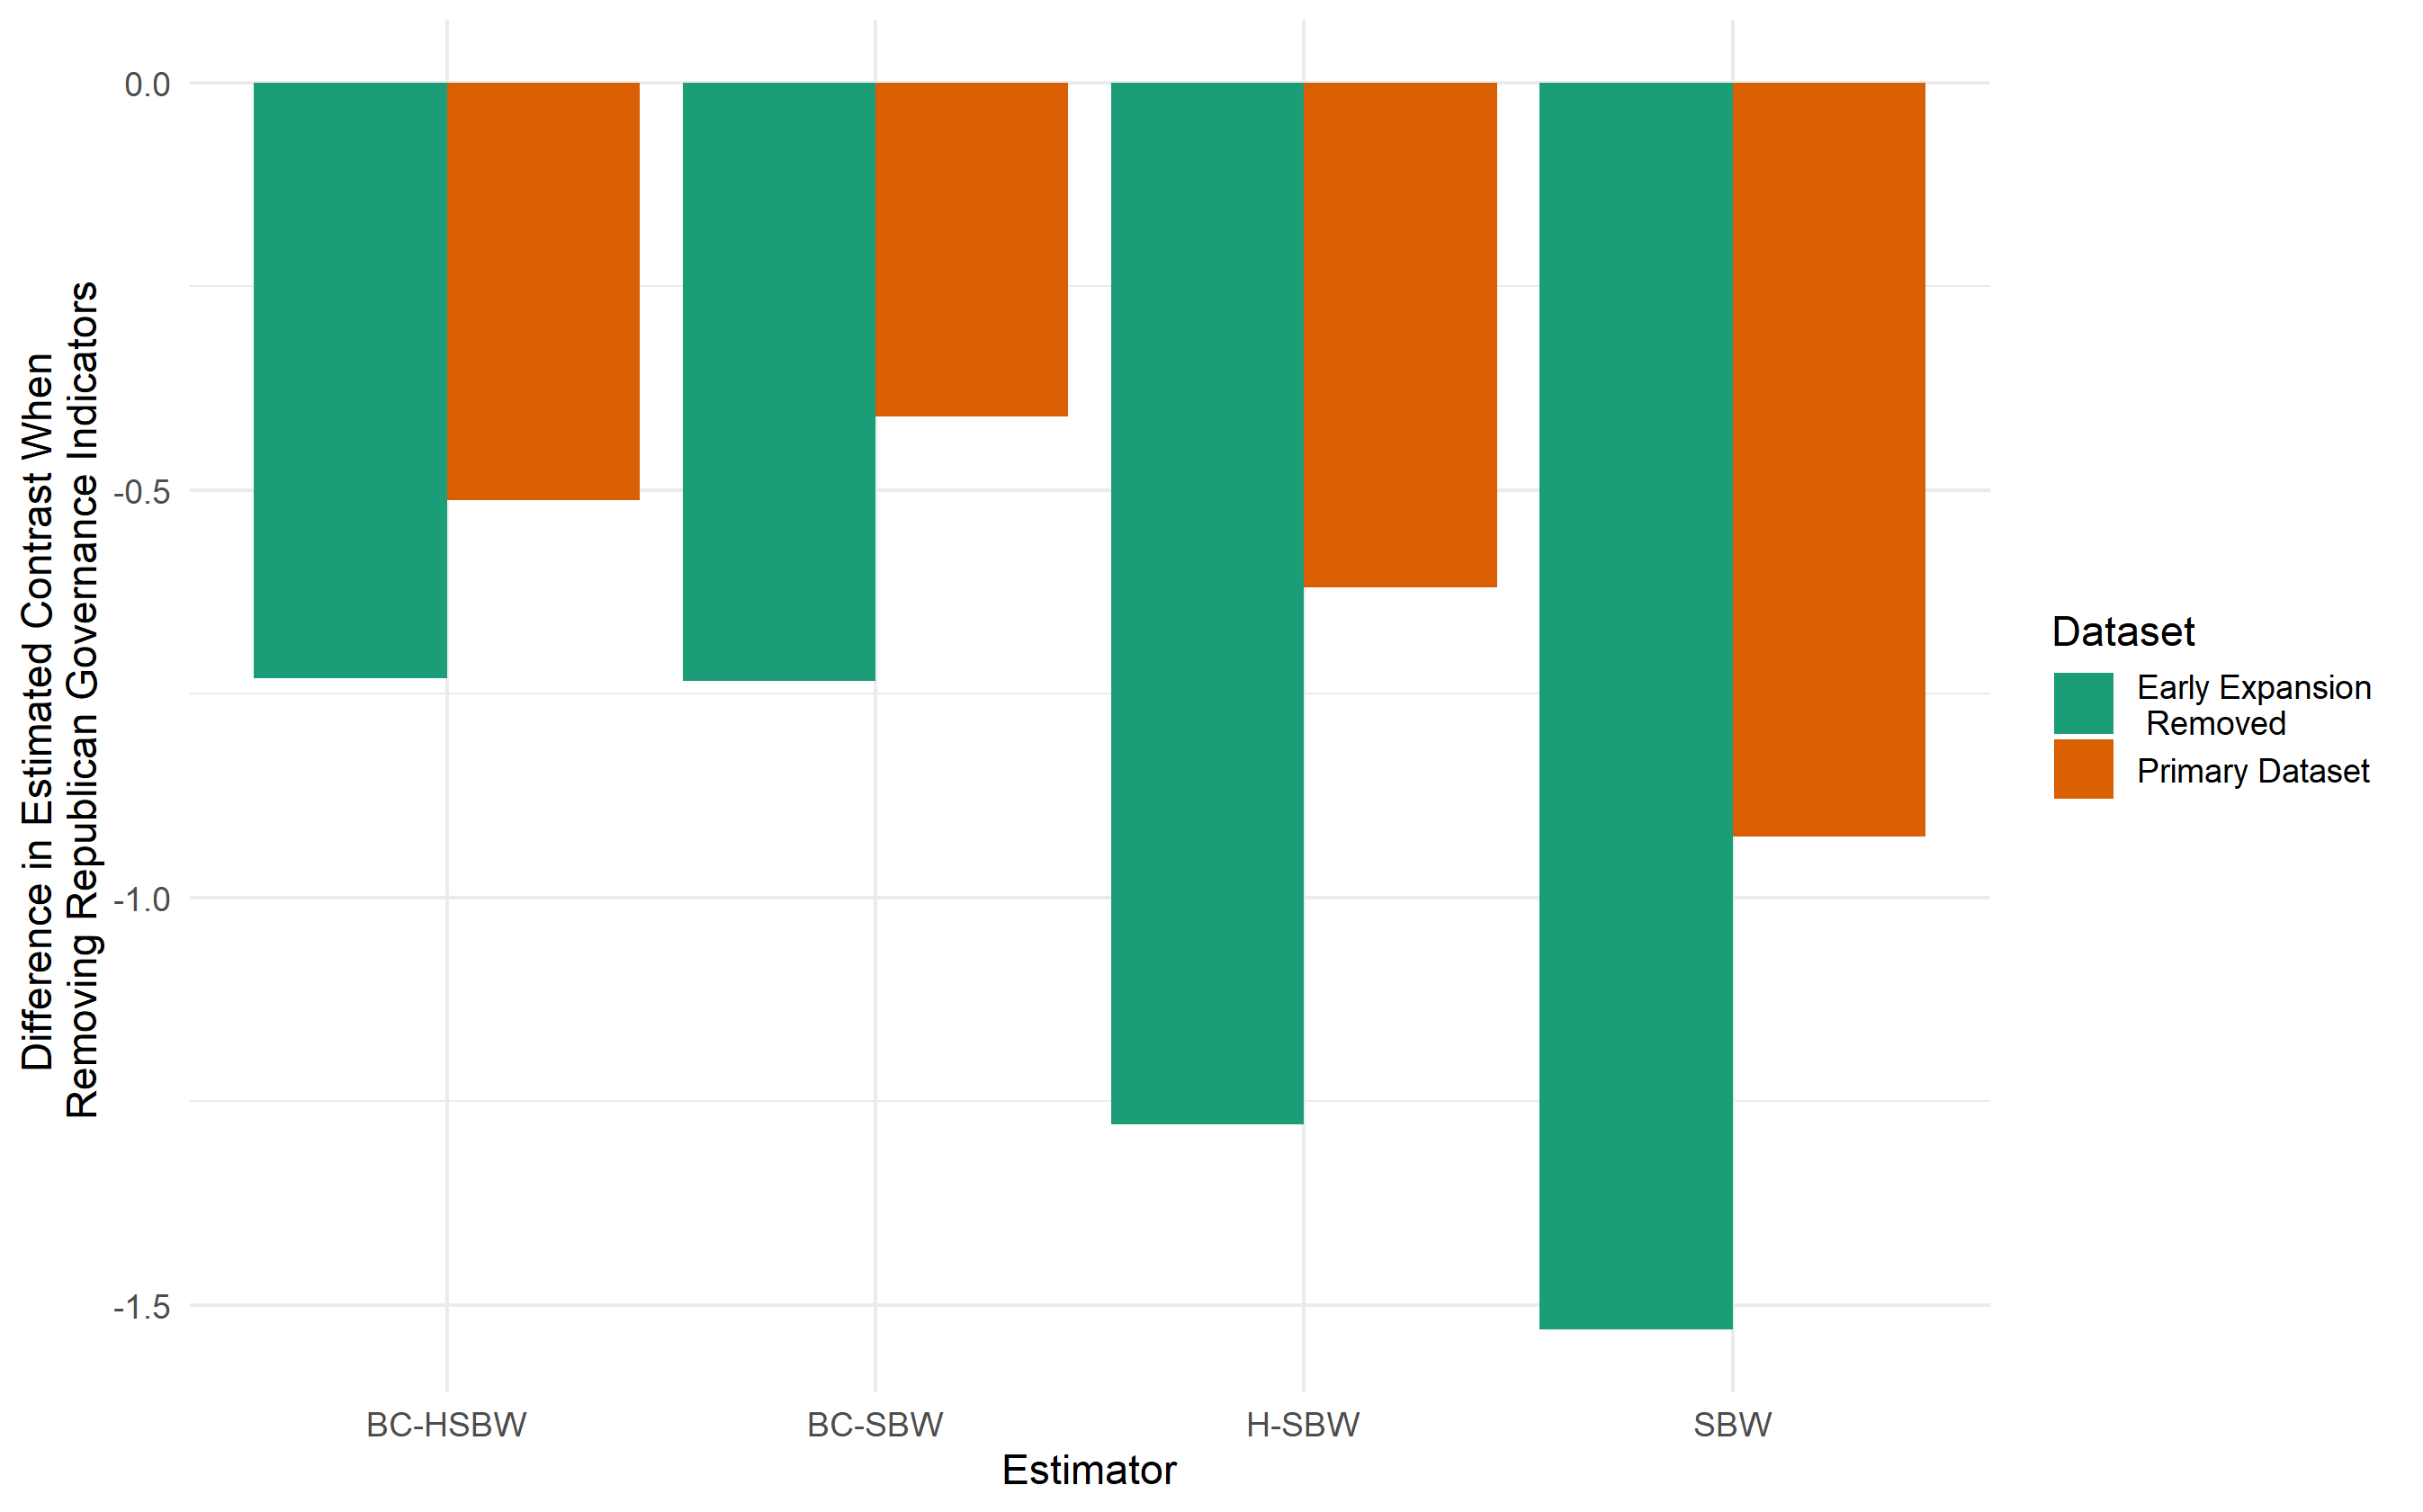
\includegraphics[scale=0.5]{01_Plots/repub-diff-c1c2.png}
    \end{center}
\end{frame}

\begin{frame}{Sensitivity analysis: OATE}
    \begin{center}
	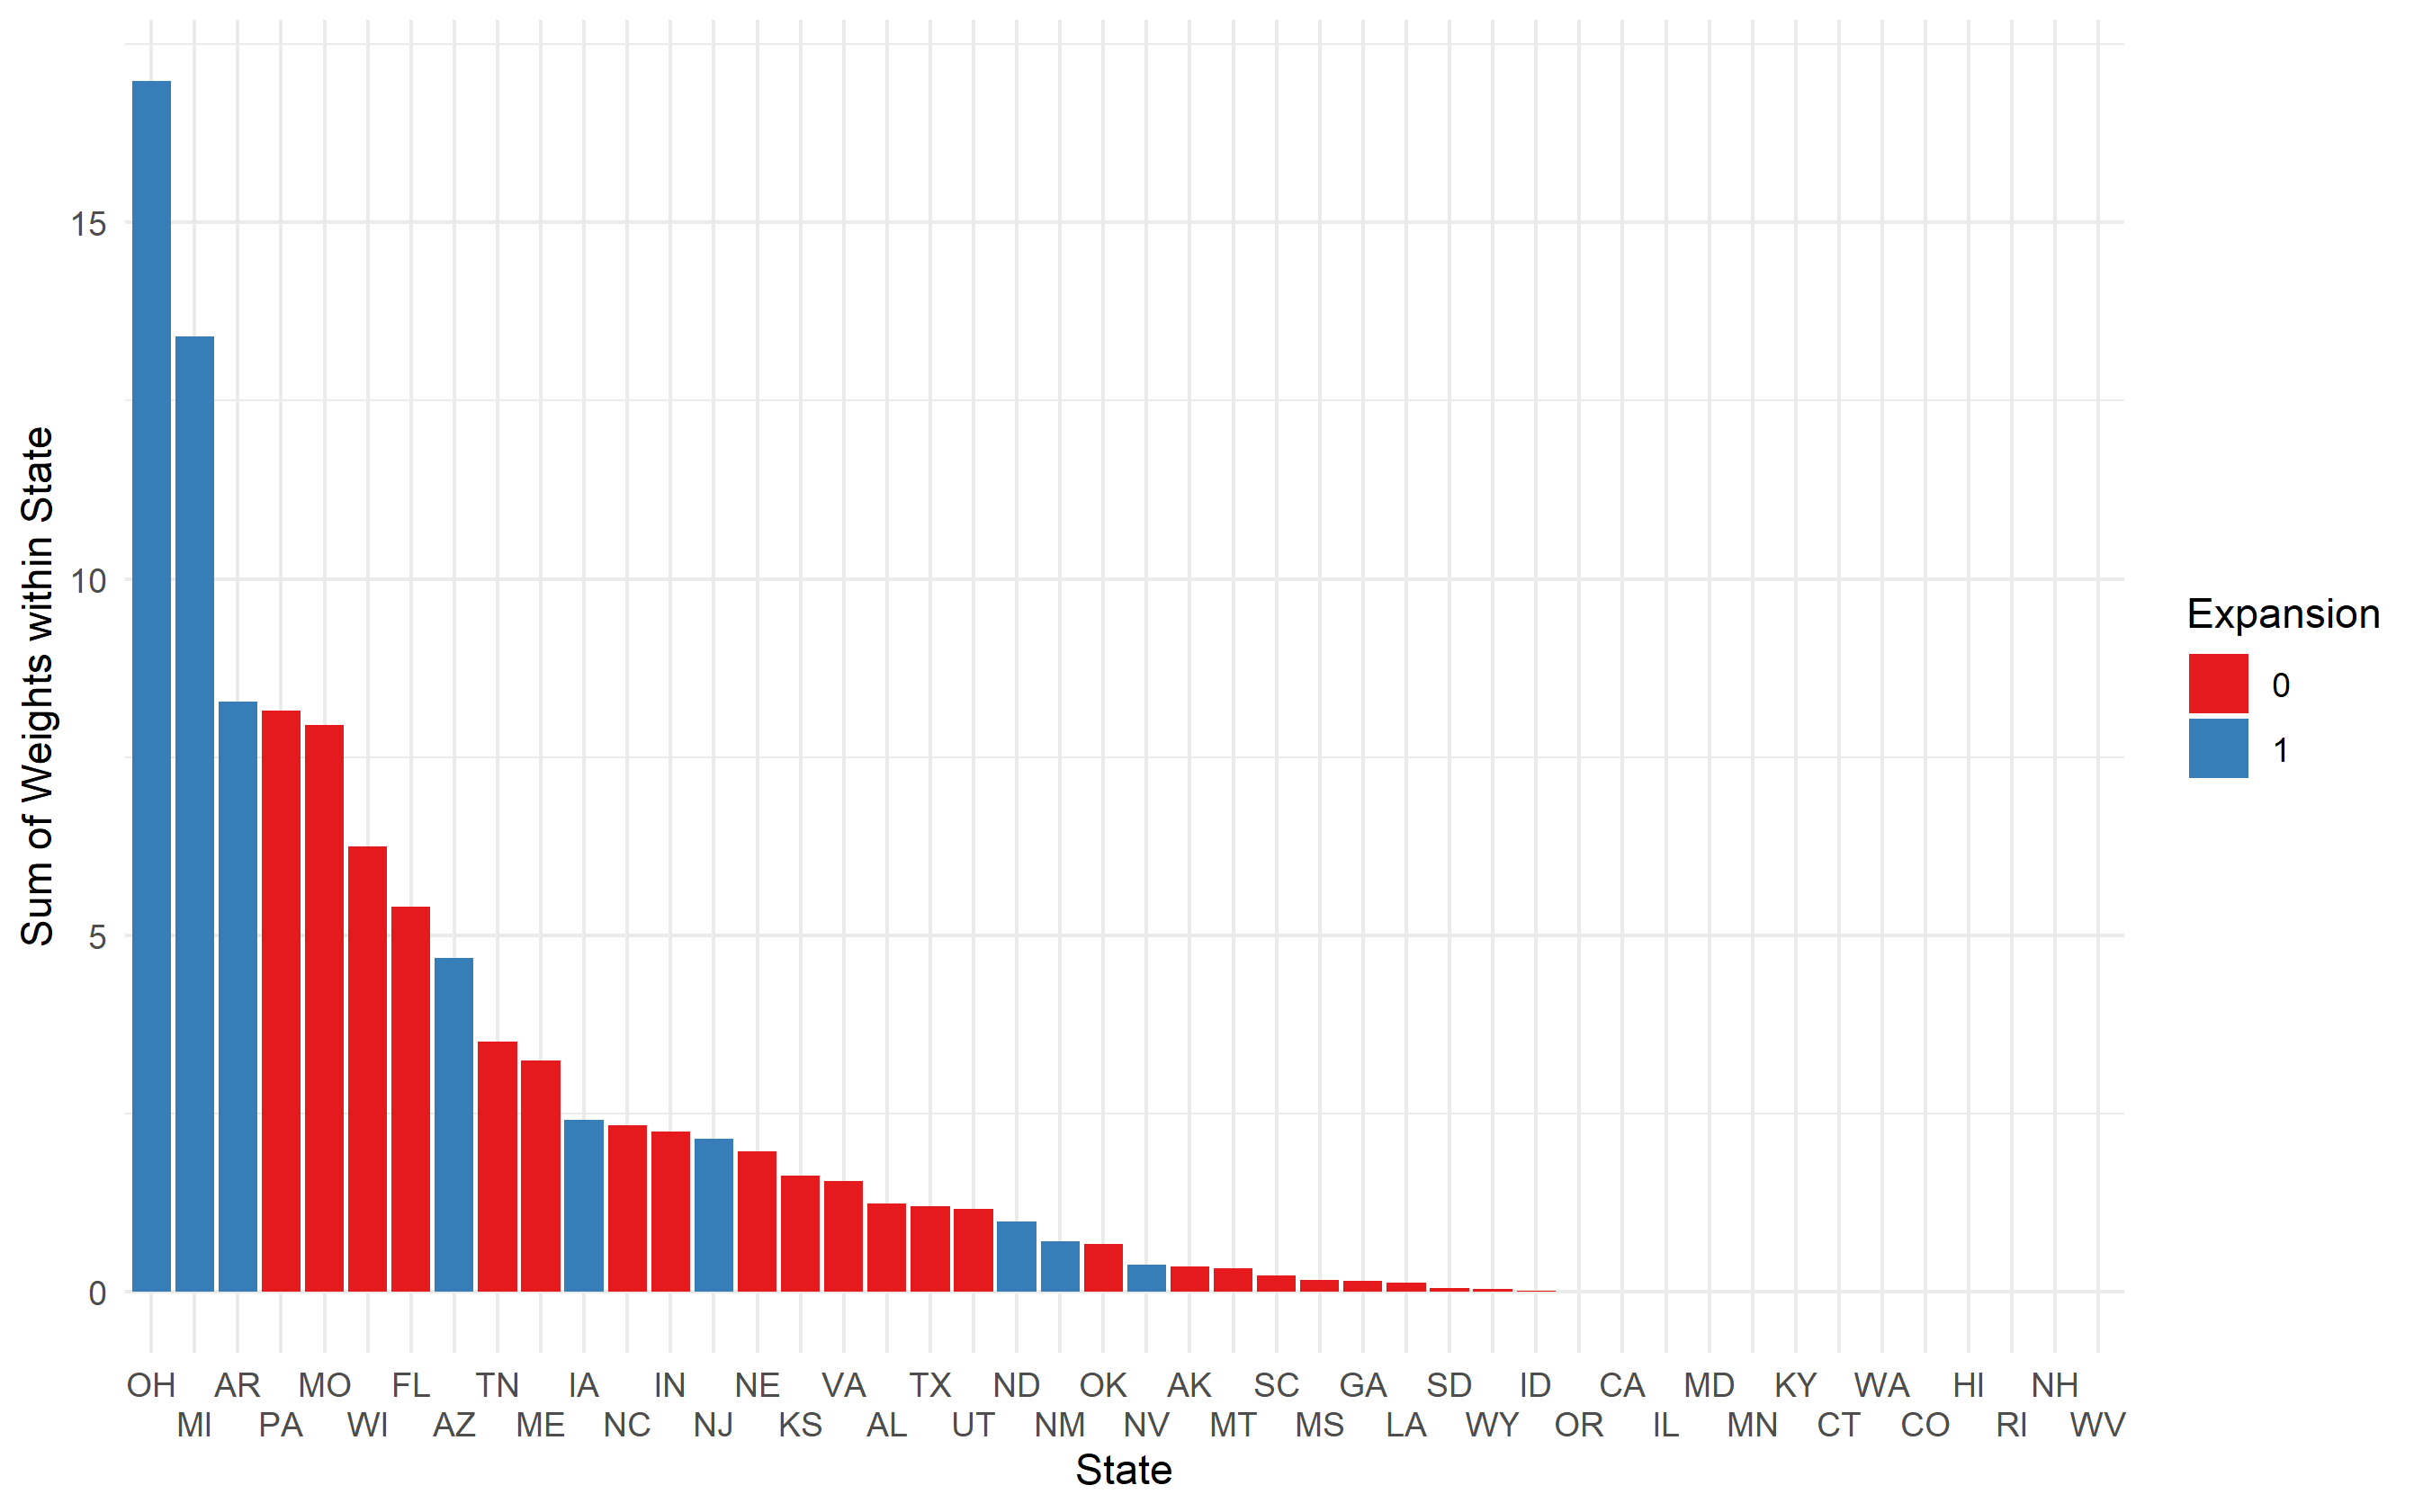
\includegraphics[scale=0.5]{01_Plots/oate-region-c1-a.png}
    \end{center}
\end{frame}

\begin{frame}{Sensitivity analysis: OATE}
INSERT OATE TABLE
\end{frame}

\begin{frame}{Sensitivity analysis: OATE}
    \begin{center}
	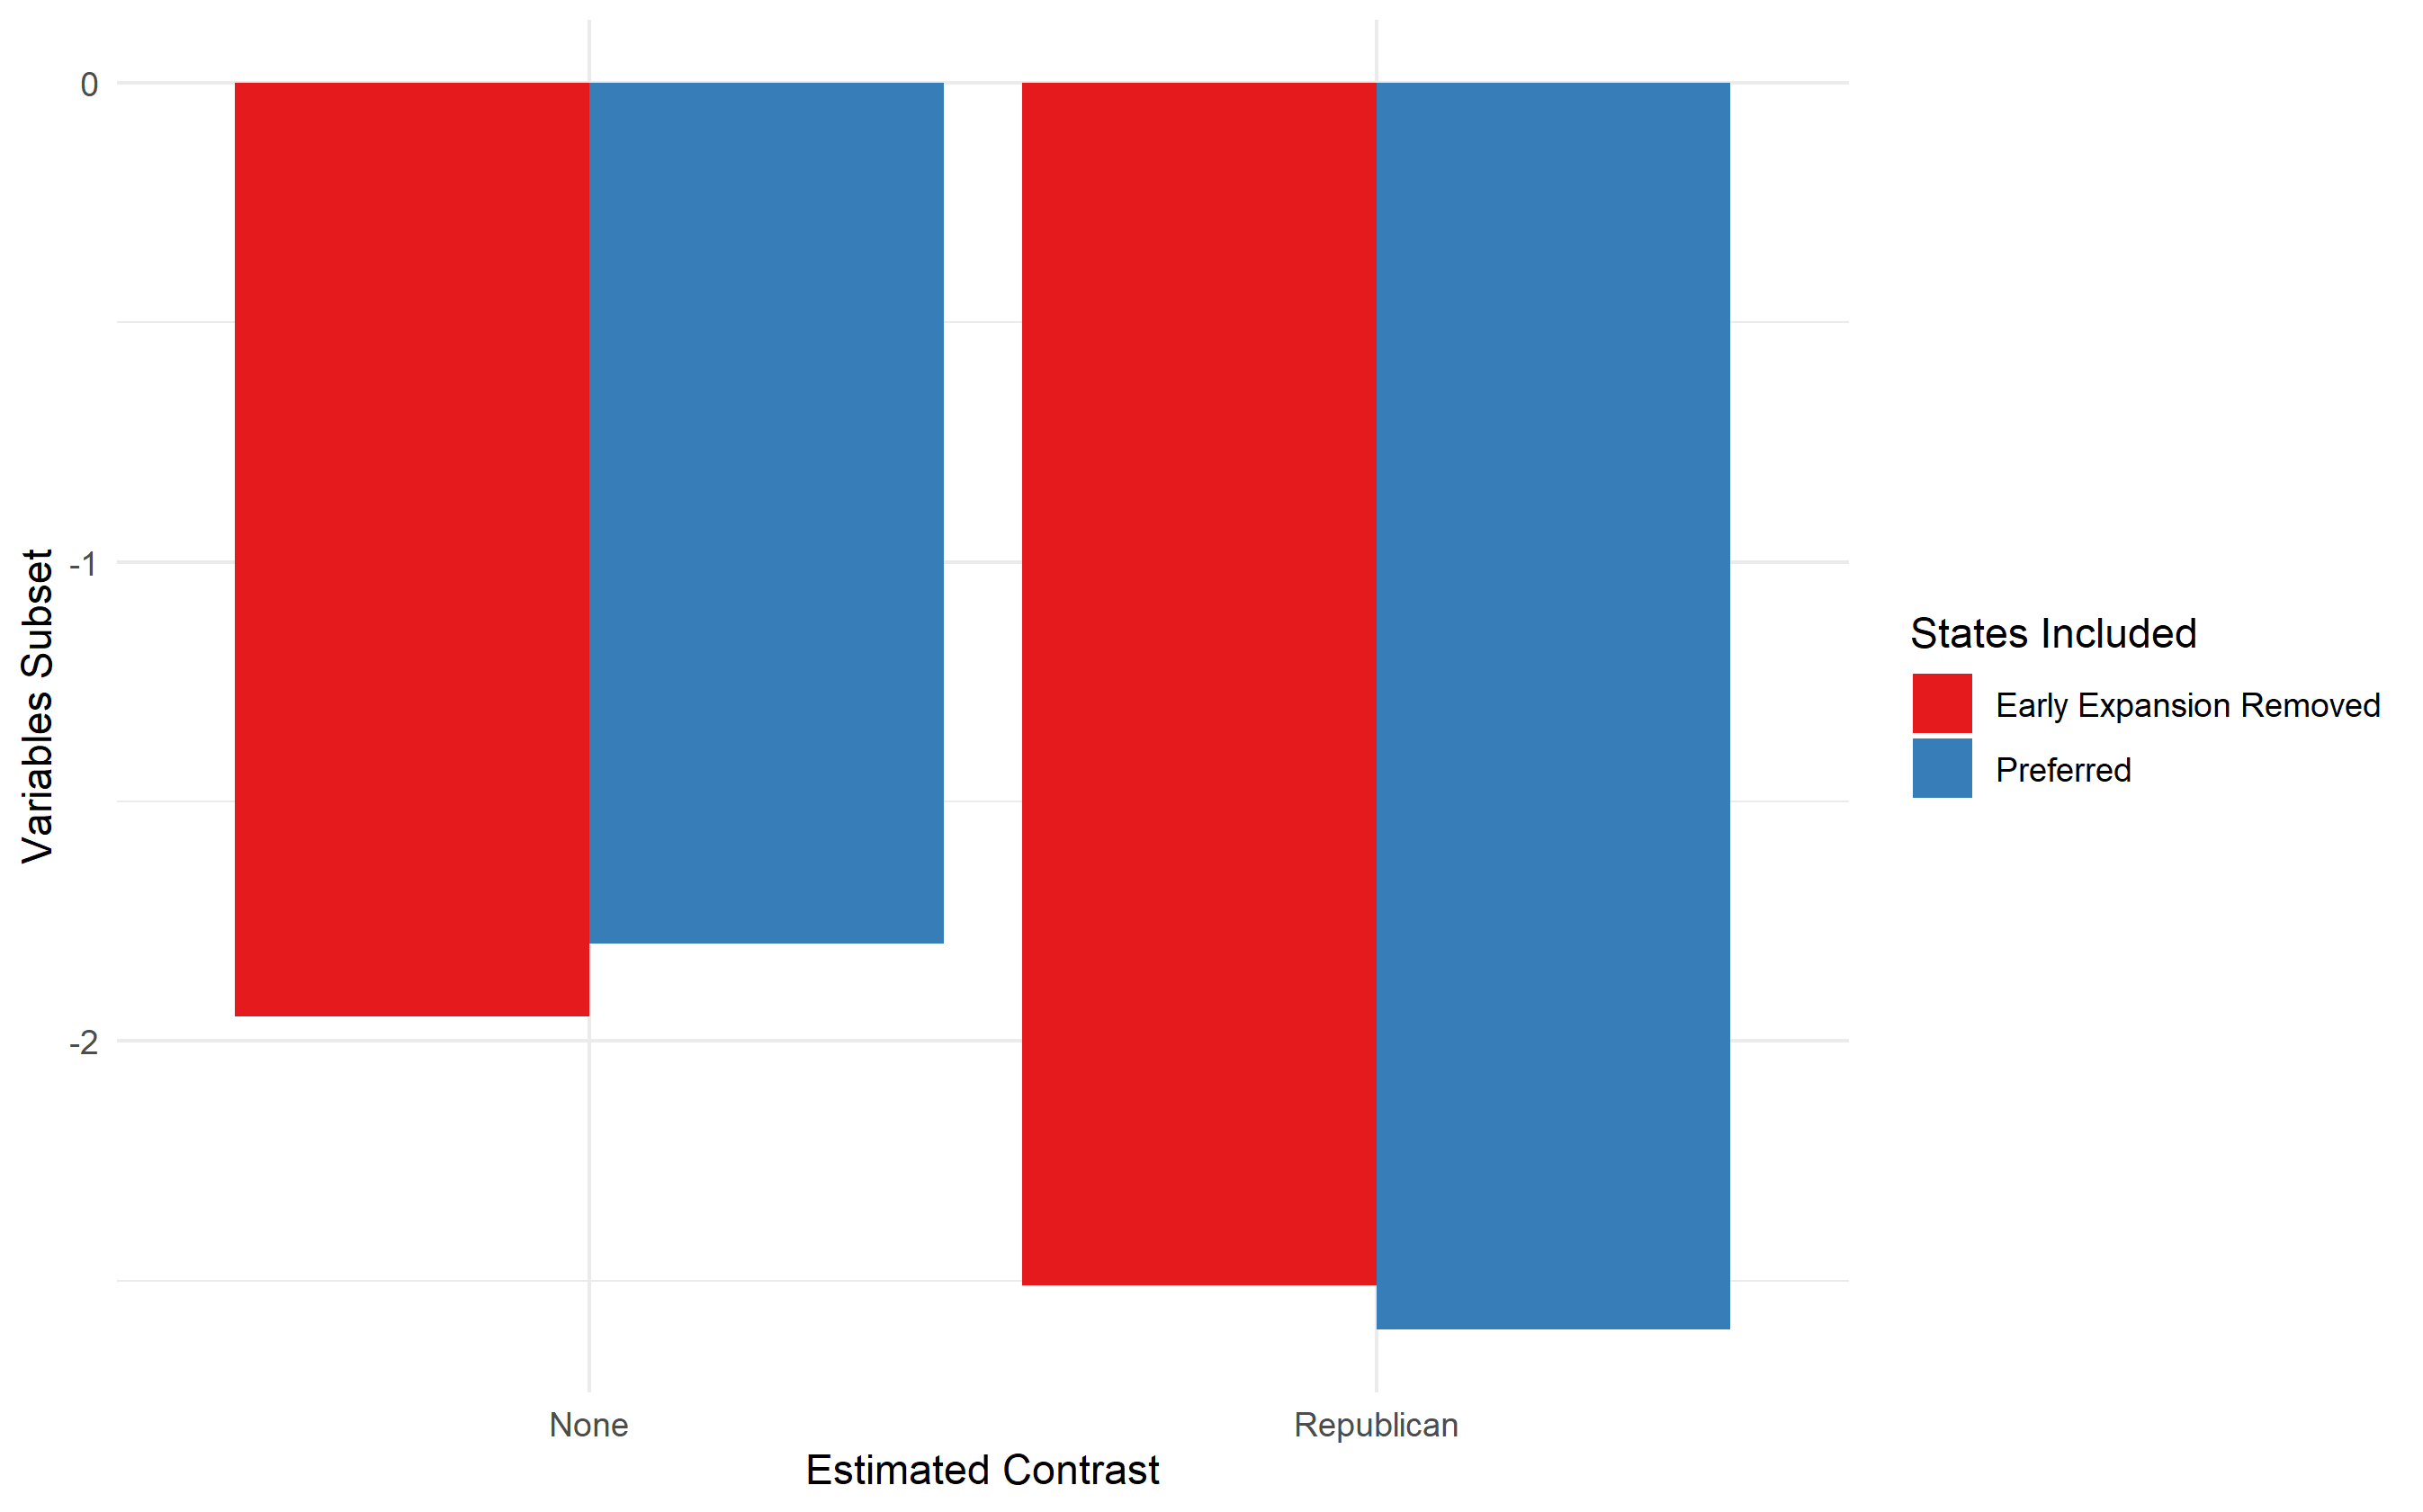
\includegraphics[scale=0.5]{01_Plots/oate-comparison-repub-c1c2.png}
    \end{center}
\end{frame}

\section{Discussion}

\subsection{Discussion}

\subsection{Discussion}

\begin{frame}{Discussion}
\begin{itemize}
    \item Propose an extension to synthetic controls to estimate the ETU \bigskip
    \item Had non-expansion states expanded Medicaid in 2014, uninsurance rates would have decreased by at most 2.08 percentage points (1.23, 2.82) \bigskip
    \item This result is robust to the exclusion of early expansion states that might introduce bias \bigskip
    \item Factors associated with Republican governance attenuate the predicted treatment effect
\end{itemize}
\end{frame}

\subsection{Conclusion}
\begin{frame}{Conclusion}
\begin{center}
Thank you for listening! \\ \newline \newline Any questions?
\end{center}
\end{frame}


\end{document}
